% \vspace{-0.2cm}
% \subsection{Implicit Regularization in Deep RL via TD-Learning}
% \vspace{-0.2cm}
\label{sec:problem}
While the ``deadly-triad''~\citep{suttonrlbook} suggests that training value function approximators with bootstrapping off-policy can lead to divergence, modern deep RL algorithms have been able to successfully combine these properties~\citep{Hasselt2018DeepRL}. However, making too many TD updates to the Q-function in offline deep RL is known to sometimes lead to performance degradation and unlearning, even for otherwise effective modern algorithms~\citep{fu2019diagnosing, fedus2020revisiting,agarwal2019optimistic,kumar2021implicit}. Such unlearning is not typically observed when training overparameterized models via supervised learning, so what about TD learning is responsible for it? We show that one possible explanation behind this pathology is the implicit regularization induced by minimizing TD error on a deep Q-network. Our theoretical results suggest that this implicit regularization ``co-adapts'' the representations of state-action pairs that appear in a Bellman backup (we will define this more precisely below).
Empirically, this typically manifests as ``co-adapted'' features for consecutive state-action tuples, even with specialized TD-learning algorithms that account for distributional shift, and this in turn leads to poor final performance both in theory and in practice. We first provide empirical evidence of this co-adaptation phenomenon in Section~\ref{app:problem_more} (additional evidence in Appendix~\ref{app:more_evidence_coadaptation}) and then theoretically characterize the implicit regularization in TD learning, and discuss how it can explain the co-adaptation phenomenon in Section~\ref{sec:theory}.


\begin{figure}[t]
    \centering
    \vspace{-5pt}
    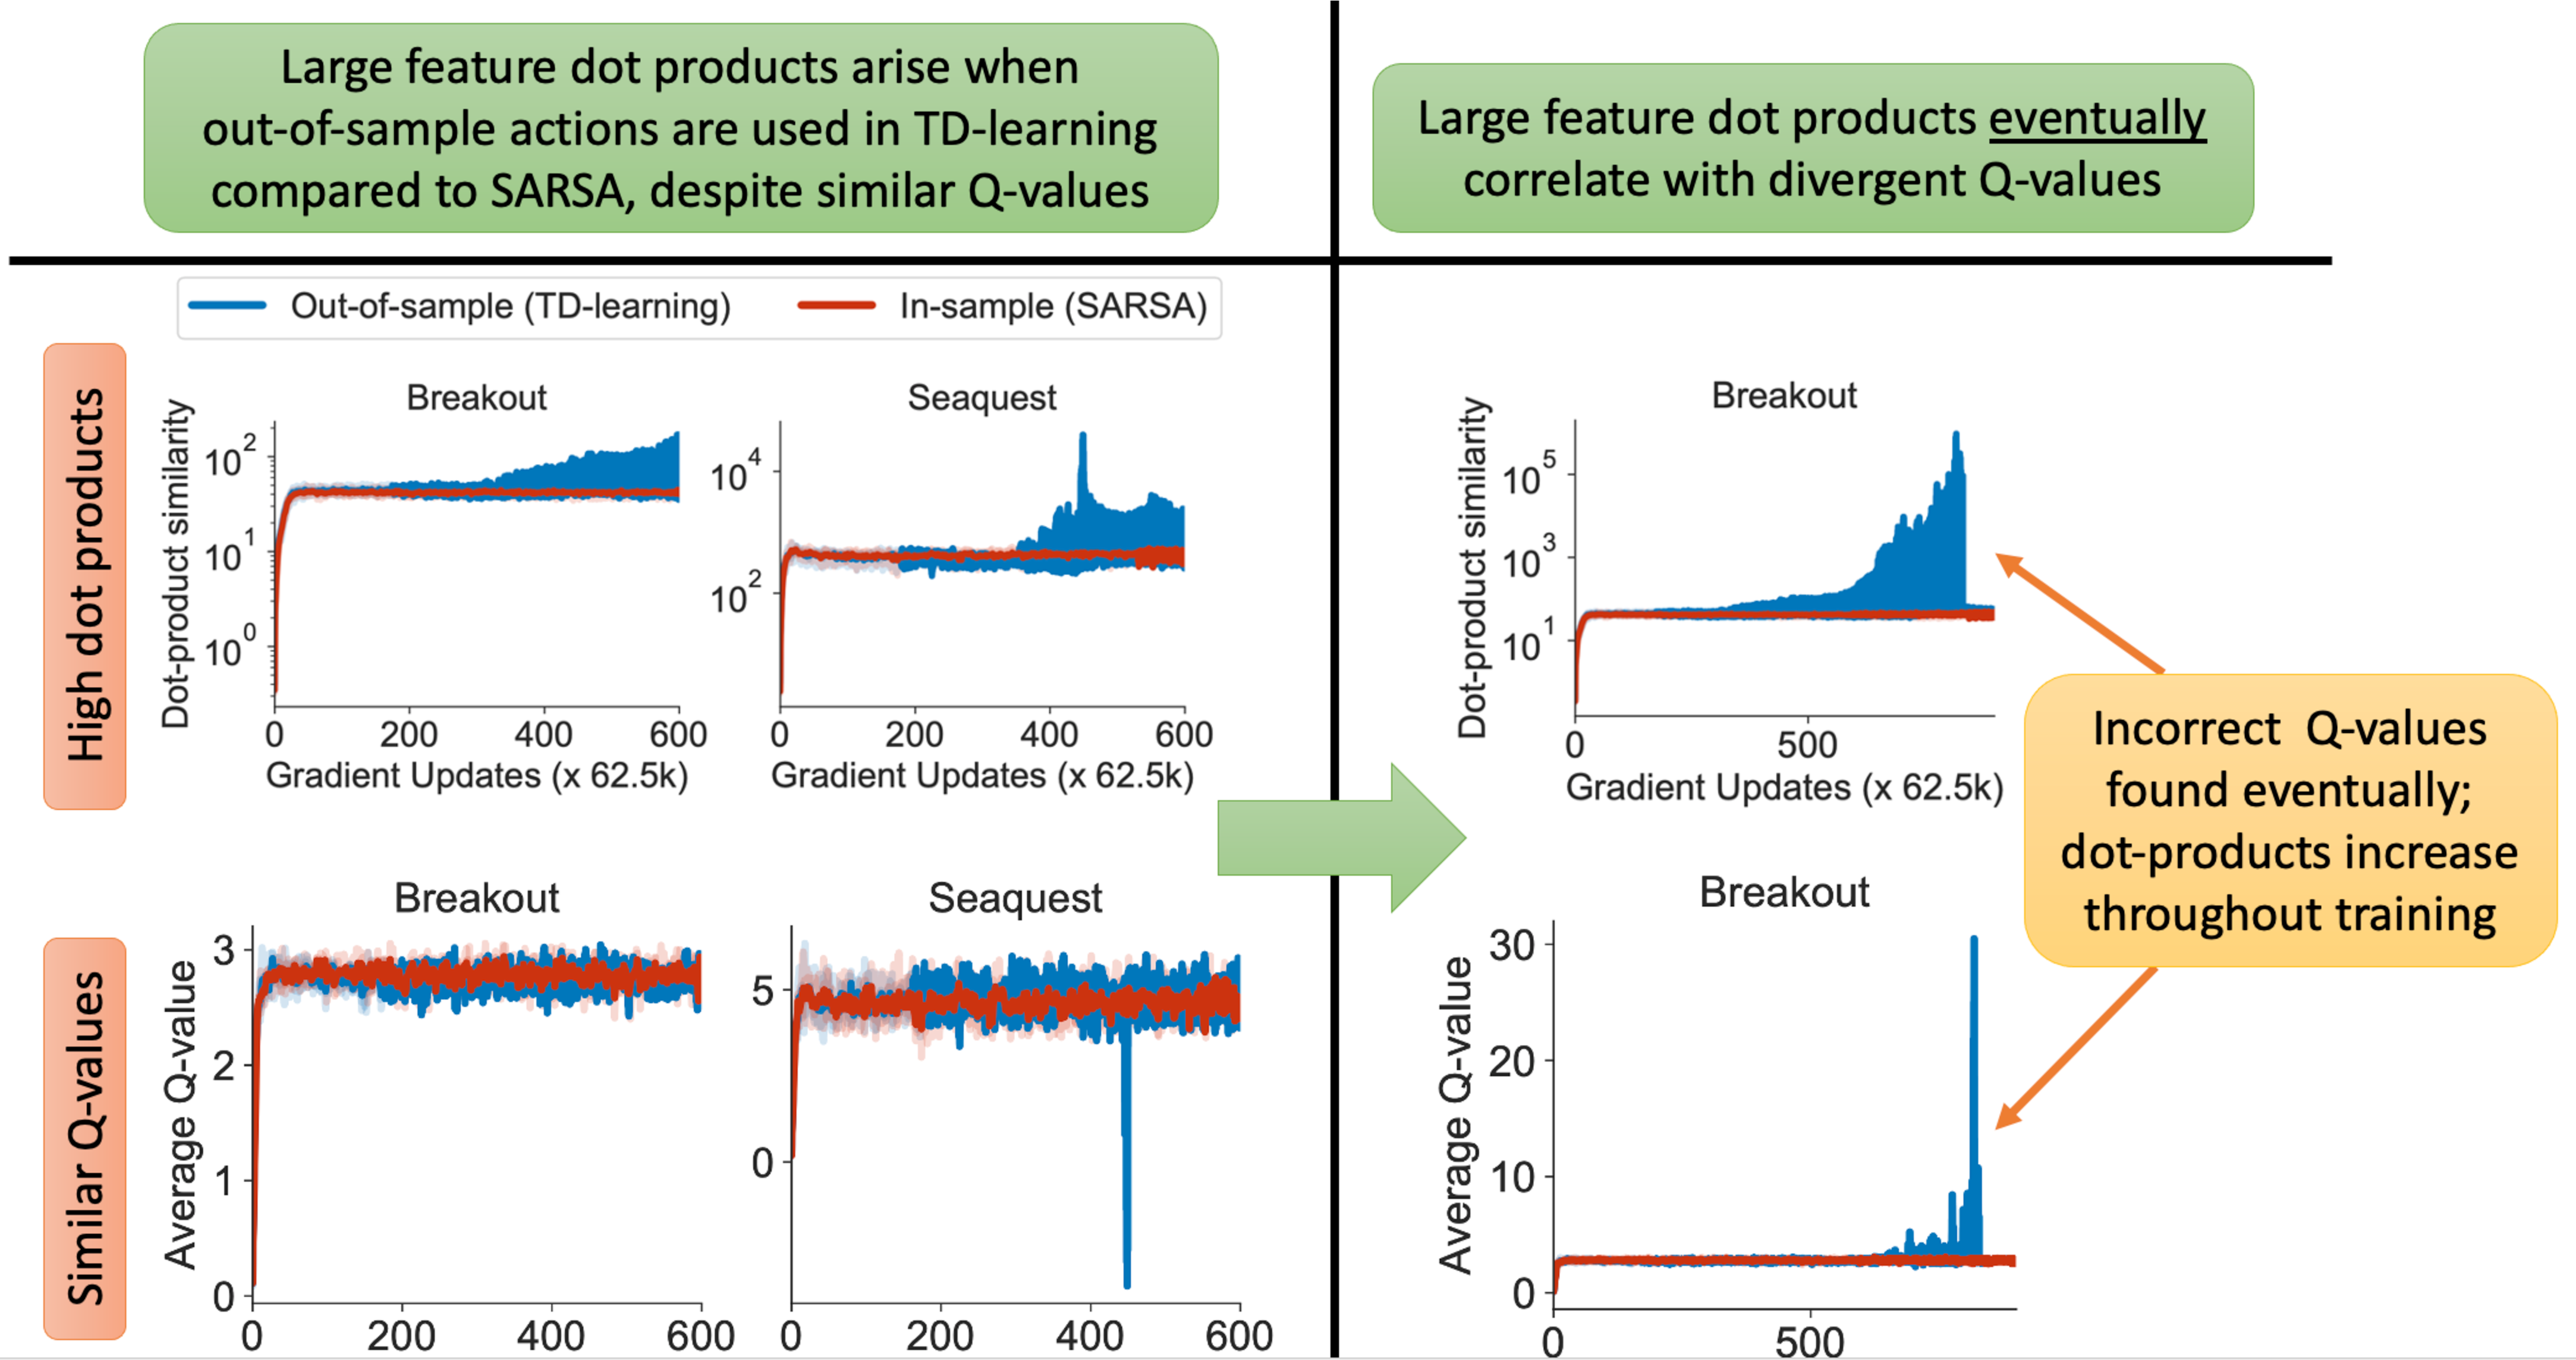
\includegraphics[width=0.67\linewidth]{chapters/dr3/figures_iclr/final_plot.pdf}~\vline~\vline~
    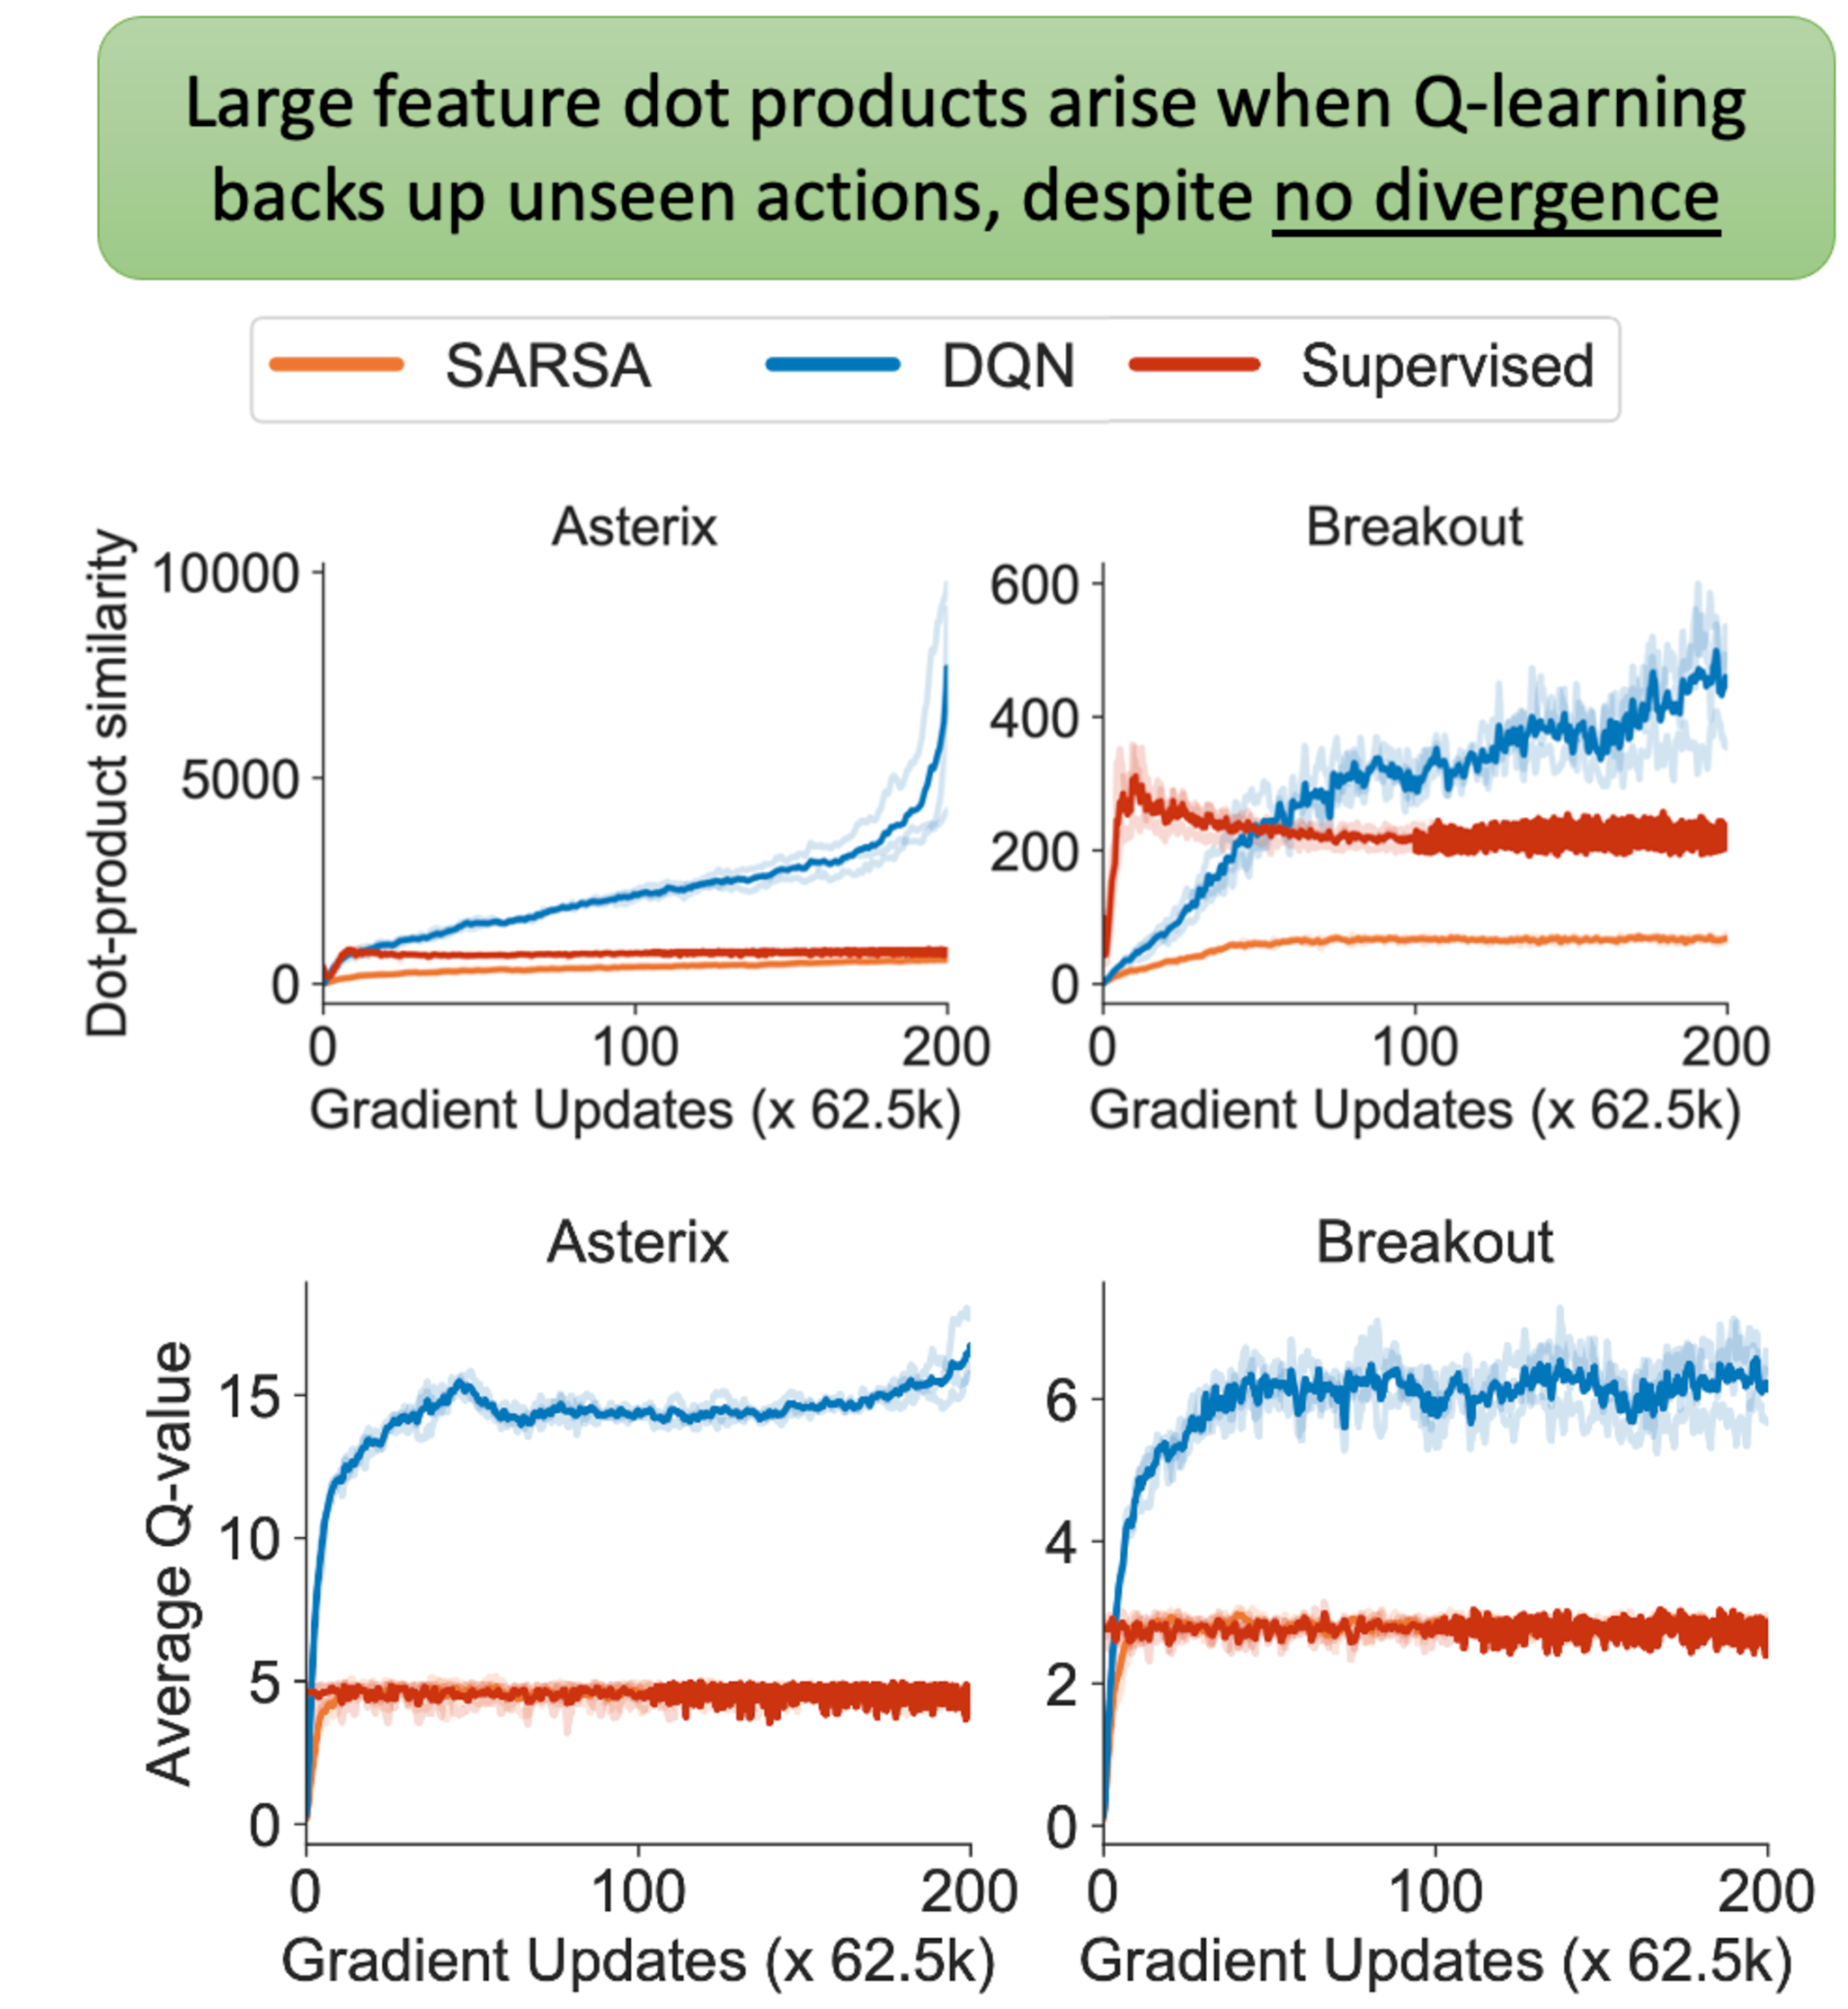
\includegraphics[width=0.32\linewidth]{chapters/dr3/figures_iclr/final_dqn_fig.pdf}
    \vspace{-0.3cm}
    \caption{\small{Feature dot-products $\phi(\bs, \mathbf{a})^\top \phi(\bs', \mathbf{a}')$ increase during training when backing up from \emph{out-of-sample} but in-distribution actions (\textbf{TD-learning}: left, \textbf{Q-learning}: right), though the average Q-value converges and stays relatively constant. Using only seen state-action pairs for backups (\textbf{offline SARSA}) or not performing Bellman backups (i.e., \textbf{supervised regression}) avoids this issue, with stable and relatively low dot products. \textit{Left}: TD-learning with high feature dot products eventually destabilizes and produces incorrect Q-values, \textit{Right}: DQN attains extremely large feature dot products, despite a relatively stable trend in Q-values.}}  
    \label{fig:dot_products}
    \vspace{-0.3cm}
\end{figure}



\subsection{Feature Co-Adaptation And Implicit Regularization}
\label{app:problem_more}

In this section, we empirically identify a \emph{feature co-adaptation} phenomenon that appears when training value functions via bootstrapping, where the feature representations of consecutive state-action pairs exhibit a large value of the dot product $\phi(\bs, \mathbf{a})^\top \phi(\bs', \mathbf{a}')$. Note that feature co-adaptation may arise because of high cosine similarity or because of high feature norms. Feature co-adaptation appears even when there is no explicit objective to increase feature similarity.

\paragraph{Experimental setup.} We ran supervised regression and three variants of approximate dynamic programming (ADP)
on an offline dataset consisting of 1\% of uniformly-sampled data from the replay buffer of DQN on two Atari games, previously used in \citet{agarwal2019optimistic}. First, for comparison, we trained a Q-function via \textbf{supervised regression} to Monte-Carlo~(MC) return estimates on the offline dataset to estimate the value of the behavior policy. Then, we trained variants of ADP which differ in the selection procedure for the action $\mathbf{a}'$ that appears in the target value in $\mathcal{L}_\mathrm{TD}(\theta)$ (Equation~\ref{eqn:td_error}). The \textbf{offline SARSA} variant aims to estimate the value of the behavior policy, $Q^{\pi_\beta}$, and sets $\mathbf{a}'$ to the actual action observed at the next time step in the dataset, such that $(\bs', \mathbf{a}') \in \mathcal{D}$. The \textbf{TD-learning} variant also aims to estimate the value of the behavior policy, but utilizes the expectation of the target Q-value over actions $\mathbf{a}'$ sampled from the behavior policy $\pi_\beta$, $\mathbf{a}' \sim \pi_\beta(\cdot|\bs')$. We do not have access to the functional form of $\pi_\beta$ for the experiment shown in Figure~\ref{fig:dot_products} since the dataset corresponds to the behavior policy induced by the replay buffer of an online DQN, so we train a model for this policy using supervised learning. However, we see similar results comparing \textbf{offline SARSA} and \textbf{TD-learning} on a gridworld domain where we can access the exact functional form of the behavior policy in Appendix~\ref{app:exact_behavior_policy}. %Unlike SARSA, this action $\mathbf{a}'$ may be different from the one in $\mathcal{D}$, though it comes from the same distribution.
All of the methods so far estimate $Q^{\pi_\beta}$ using different target value estimators.
We also train \textbf{Q-learning}, which chooses the action $\mathbf{a}'$ to maximize the learned Q-function. While Q-learning learns a different Q-function, we can still compare the relative stability of these methods to gain intuition about the learning dynamics. %To measure feature co-adaptation, we track the average dot product between the learned features at consecutive state-action tuples, $\text{sim}(\bs, \mathbf{a}, \bs', \mathbf{a}') := \phi(\bs, \mathbf{a})^\top \phi(\bs', \mathbf{a}')$. 
In addition to feature dot products $\phi(\bs, \mathbf{a})^\top \phi(\bs', \mathbf{a}')$, we also track the average prediction of the Q-network over the dataset to measure whether the predictions diverge or are stable in expectation.

%%AK: also need to figure out an arrangement for figures in the paper
\paragraph{Observing feature co-adaptation empirically.} As shown in Figure~\ref{fig:dot_products} (right), the average dot product (top row) between features at consecutive state-action tuples continuously increases for both Q-learning and TD-learning (after enough gradient steps), whereas it flatlines and converges to a small value for supervised regression. We might at first think that this is simply a case of Q-learning failing to converge. However, the bottom row shows that the average Q-values do in fact converge to a stable value. Despite this, the optimizer drives the network towards higher feature dot products. There is no explicit term in the TD error objective that encourages this behavior, 
% and in fact the TD error relatively stays flat \textcolor{red}{(Figure ??)} during training, 
indicating the presence of some implicit regularization phenomenon. This \emph{implicit} preference towards maximizing the dot products of features at consecutive state-action tuples is what we call ``feature co-adaptation.''

\paragraph{When does feature co-adaptation emerge?} Observe in Figure~\ref{fig:dot_products} (right) that the feature dot products for offline SARSA converge quickly and are relatively flat, similarly to supervised regression. This indicates that utilizing a bootstrapped update alone is not responsible for the increasing dot-products and instability, because while offline SARSA uses backups, it behaves similarly to supervised MC regression. Unlike offline SARSA, feature co-adaptation emerges for TD-learning, which is surprising as TD-learning also aims to estimate the value of the behavior policy, and hence should match offline SARSA in expectation. The key difference is that while offline SARSA always utilizes actions $\mathbf{a}'$ observed in the training dataset for the backup, TD-learning may utilize potentially unseen actions $\mathbf{a}'$ in the backup, even though these actions $\mathbf{a}' \sim \pi_\beta(\cdot|\bs')$ are \emph{within} the distribution of the data-generating policy. This suggests that utilizing \textbf{out-of-sample} actions in the Bellman backup, even when they are not out-of-distribution, critically alters the learning dynamics. This is distinct from the more common observation in offline RL, which attributes training challenges to out-of-distribution actions, but not out-of-sample actions. The theoretical model developed in Section~\ref{sec:theory} will provide an explanation for this observation with a discussion about how feature co-adaption caused due to out-of-sample actions can be detrimental in offline RL. 

% While action $\mathbf{a}'$ can be out-of-distribution in the case of Q-learning, this action is sampled from the data-generating distribution of the behavior policy for TD-learning and is hence, not out-of-distribution in this case.

%%AK: does it feel like a jump here, or is it fine?
% The only difference between offline SARSA and Q-learning is whether unseen actions are used to compute the Bellman target\gjt{I don't think that is an accurate statement. The action selection mechanism is different.}:
%%SL.9.17: Yeah, this is correct. Maybe it would be better to mention the TD thing as well in the first paragraph, rather than introducing it for the first time in this paragraph below? That would avoid one very likely criticism you would otherwise get about the comparison between SARSA and Q-learning being non-sensical because they are just learning totally different things
% while $(\bs', \mathbf{a}')$ used in Q-learning may be unobserved in $\mathcal{D}$, the $(\bs', \mathbf{a}')$ tuples used in SARSA appear in the dataset, i.e., $(\bs', \mathbf{a}') \in \mathcal{D}$÷.
%%SL.9.17: some readers won't understand why
% Thus, we might wonder if the use of OOD actions in the backup is the primary culprit for the difference in the observed trends. 

% To understand if this is the case, in Figure~\ref{fig:dot_products} (left), we compare offline SARSA to another variant that we call \textbf{TD-learning},
% %%AK: need to rename TD-learning to something else?
% which utilizes potentially unseen but in-distribution actions sampled from the behavior policy for the Bellman update, such that $\mathbf{a}' \sim \pi_\beta(\cdot|\bs')$. Like offline SARSA, TD-learning also aims to estimate the value of the behavior policy $Q^{\pi_\beta}$, but it differs from offline SARSA in that the actions $\mathbf{a}'$ are sampled from the data-generating distribution of the behavior policy. Thus, while they are not \emph{out-of-distribution}, they are also generally not actions that were seen in the dataset $\mathcal{D}$, in contrast to offline SARSA.
% %%SL.9.17: This paragraph is already really hard to read, adding a footnote that creates another branch point for the reader creates an overwhelming cognitive load. Try to merge this footnote into the paragraph, and generally just shorter, more concise, and more digestible sentences.
% % to compute the value of the behavior policy $Q^{\pi_\beta}$. \textbf{Offline SARSA} and \textbf{TD-learning} should match in expectation. 
% As expected, we observe in Figure~\ref{fig:dot_products} (left) that the Q-values predicted by TD-learning match those learned by \textbf{offline SARSA}. However, in contrast to \textbf{offline SARSA}, we find that the dot product similarity for TD-learning increases after enough gradient steps, and this is accompanied by instability in the Q-values. This trend is absent in offline SARSA. This suggests that utilizing out-of-sample actions (even when they are not OOD) in the Bellman backup critically alters the learning dynamics. The theoretical model developed in Section~\ref{sec:theory} provides an explanation for this observation. 
%%AK: one concern: we overload "TD-learning" to mean generic bootstrapping algorithms as well as the "TD learning" baseline we plot. Should we change one of them to something else? Like calling TD-learning generically as bootstrapping and TD learning baseline as FQE.

%%SL.9.17: You can probably shorten this paragraph if you want to save some space
 
% What is the implicit mechanism causing co-adaptation, and why does it occur only when using out-of-sample state-action tuples for the backup? This issue is not corrected by existing offline RL methods, which only avoid out-of-distribution actions~\citep{levine2020offline}, so how does co-adaptation affect offline RL performance? In the next section, we will show how an implicit regularization effect that is studied as a potential benefit of SGD in supervised deep learning can explain this phenomenon, and how this leads to a number of issues in the RL setting.

% \textbf{How do Bellman backups with out-of-sample actions behave?} 
% As shown in Figure~\ref{fig:dot_products} (left), with \textbf{TD-learning}, the dot products steadily increase during training though the average Q-value predictions are roughly constant over the this phase. These Q-values on average match those learned by \textbf{offline SARSA} and \textbf{supervised regression},
% %%SL.7.13: Supervised regression doesn't appear in the left plots!
% but the dot products for \textbf{SARSA} and supervised learning remain flat. In contrast, with \textbf{TD-learning}, the dot products increase after too many gradient steps, and this is accompanied by instability in the Q-values, which then diverge. Note that the only difference between \textbf{TD-learning} and \textbf{SARSA} is the resampling of the target value action, where \textbf{TD-learning} uses a new (out-of-sample) action from the same distribution, while \textbf{SARSA} uses the dataset action.
% %these two approaches quickly converge over the course of training unlike \textbf{TD-learning}. With more training, we find that \textbf{TD-learning} exhibits unstable Q-values, which eventually diverge, whereas the predictions for both \textbf{offline SARSA} and \textbf{supervised regression} converge and do not destabilize with more training.
% % Notably, with \textbf{TD-learning}, the dot-products steadily increase during training and the Q-values eventually diverge, whereas both the dot-products and Q-values of \textbf{offline SARSA} and \textbf{supervised regression} quickly converge and remain stable throughout training (Figure 2). 
% These observations indicate that Bellman backups alone are not responsible for the increasing dot-products and instability because \textbf{offline SARSA} uses Bellman backups, but behaves similarly to \textbf{supervised regression}.
% %%SL.7.13: Again, this is not apparent from the figure, because supervised regression is not shown on the left side!
% On the other hand, \textbf{TD-learning}, which uses out-of-sample actions in the Bellman backup, exhibits increasing dot-products, which eventually ends in  instability, suggesting that out-of-sample actions critically alter the learning dynamics. The theoretical model developed in Section~\ref{sec:theory} provides an explanation for this observation.

% Next, we train two methods that estimate the value of the behavior policy that generated the dataset via dynamic programming. The first approach, which we refer to as  standard \textbf{TD-learning}, estimates $Q^{\pi_\beta}$ by minimizing TD-error $\mathcal{L}_\mathrm{TD}(\theta)$ (Equation in Section~\ref{sec:background}), 
% % $\sum_{\bs, \mathbf{a}, \bs' \in \mathcal{D}, \mathbf{a}' \sim {\pi}_\beta(\cdot | \bs')} \left(R(\bs, \mathbf{a}) + \gamma \mathbf{a}r{Q}_\theta(\bs', \mathbf{a}') - Q_\theta(\bs, \mathbf{a}) \right)^2$, 
% where the action $\mathbf{a}' \sim {\pi}_\beta(\cdot|\bs)$ is sampled from the behavior policy and can be \textit{out-of-sample} for the training dataset, i.e., $(\bs', \mathbf{a}') \notin \mathcal{D}$, but is \emph{in-distribution}. \aviral{This version is implemented by first learning a model of the behavior policy using supervised classification.} The second approach, which we refer to as \textbf{offline SARSA}, performs Bellman backups from the exact $(\bs', \mathbf{a}')$ tuple observed in the dataset $\mathcal{D}$ (i.e., $\mathbf{a}'$ appearing in $\mathcal{L}_\mathrm{TD}(\theta)$ is observed in $\mathcal{D}$).
% % minimizing $\sum_{\bs, \mathbf{a}, \bs', \mathbf{a}' \in \mathcal{D}} \left(R(\bs, \mathbf{a}) + \gamma \mathbf{a}r{Q}_\theta(\bs', \mathbf{a}') - Q_\theta(\bs, \mathbf{a}) \right)^2$). 
% Offline SARSA is the same as TD-learning in expectation. However, TD-learning uses potentially out-of-sample actions\footnote{Note that these actions are sampled from the data generating distribution, hence are not out-of-distribution, but may be absent from the training dataset.} in the backup.   As we will show, utilizing out-of-sample state-action tuples in the backup plays a critical role in the learning dynamics.
% Finally, we also train standard \textbf{Q-learning}, which chooses actions $\mathbf{a}'$ that maximize the learned Q-function. Such actions are also out-of-sample.  


%%SL.7.13: My high-level comment on this section is the following: Right now, your analysis launches into the out-of-sample action discussion right away, without adequately explaining feature co-adaptation. This feels like it's putting the cart before the horse -- before the reader has fully appreciated or even understood what co-adaptation means, they are confronted with this somewhat nuanced discussion about out-of-sample actions. Maybe we should have a couple of sentences before this that basically say "notice how the feature dot products tend to go up right around the same time that things get unstable, isn't that funny? this is what we call feature co-adaptation, let's see what kinds of methods have this issue, and what kinds don't" -- this could be written in just a few sentences, and it should come *before* the discussion of out-of-sample actions, which is secondary to this.


% \begin{figure}[t]
%     \centering
%     \vspace{-5pt}
%     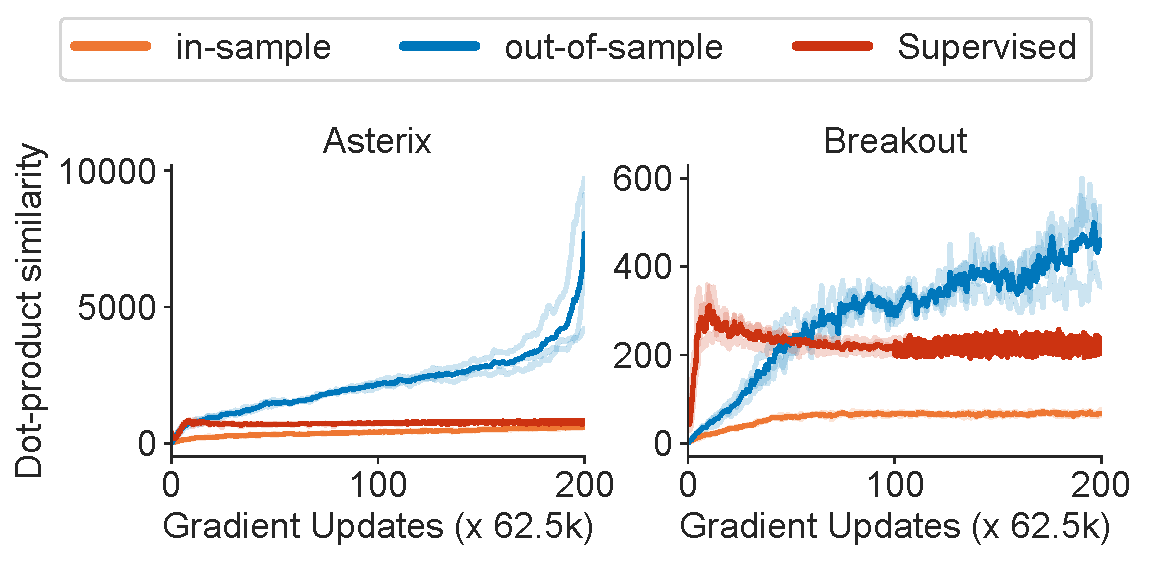
\includegraphics[width=0.45\linewidth]{figures/figure1_dotproduct_dot_products_final.pdf}\\
%     ~~~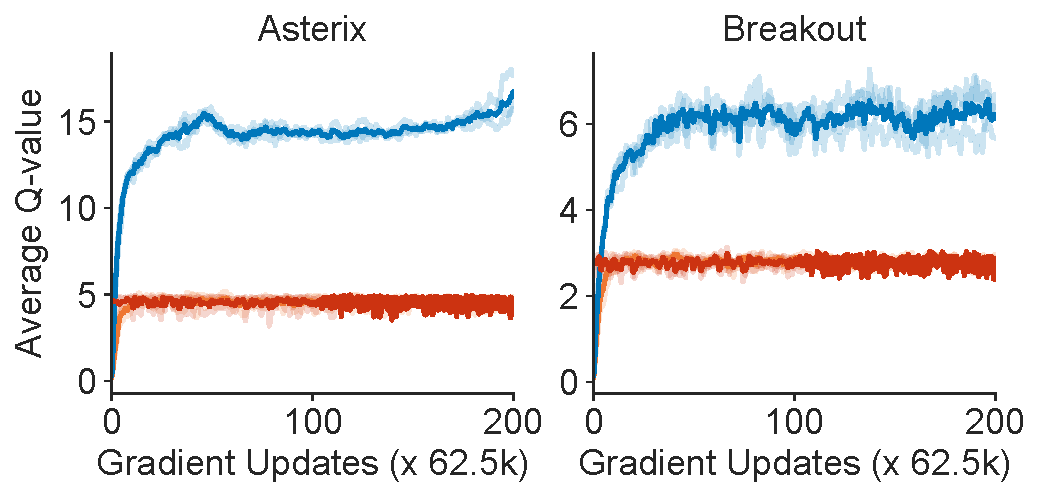
\includegraphics[width=0.45\linewidth]{section3_figs/figure1_dotproduct_q_values (1).pdf}
%     \vspace{-0.24cm}
%     %%SL.5.22: Let's not label it "MC", that's not very informative. Call it "supervised" instead.
%     %%AK: TODO for me, will change it. 
%     %%AK: change labels here
%     \caption{\small{Dot-product $\text{sim}(\bs, \mathbf{a}, \bs', \mathbf{a}')$ increases through training when backing up from out-of-sample actions though the average Q-value stays relatively constant, whereas utilizing seen state-action pairs for backups or supervised learning exhibit near-constant dot product similarities as well.}}  
%     \label{fig:dot_products}
%     \vspace{-0.6cm}
% \end{figure}
% \textbf{How do Bellman backups with out-of-sample actions behave?} 
% As shown in Figure~\ref{fig:dot_products} (left), with \textbf{TD-learning}, the dot products steadily increase during training though the average Q-value predictions are roughly constant over the this phase. These Q-values on average match those learned by \textbf{offline SARSA} and \textbf{supervised regression},
% %%SL.7.13: Supervised regression doesn't appear in the left plots!
% but the dot products for \textbf{SARSA} and supervised learning remain flat. In contrast, with \textbf{TD-learning}, the dot products increase after too many gradient steps, and this is accompanied by instability in the Q-values, which then diverge. Note that the only difference between \textbf{TD-learning} and \textbf{SARSA} is the resampling of the target value action, where \textbf{TD-learning} uses a new (out-of-sample) action from the same distribution, while \textbf{SARSA} uses the dataset action.
% %these two approaches quickly converge over the course of training unlike \textbf{TD-learning}. With more training, we find that \textbf{TD-learning} exhibits unstable Q-values, which eventually diverge, whereas the predictions for both \textbf{offline SARSA} and \textbf{supervised regression} converge and do not destabilize with more training.
% % Notably, with \textbf{TD-learning}, the dot-products steadily increase during training and the Q-values eventually diverge, whereas both the dot-products and Q-values of \textbf{offline SARSA} and \textbf{supervised regression} quickly converge and remain stable throughout training (Figure 2). 
% These observations indicate that Bellman backups alone are not responsible for the increasing dot-products and instability because \textbf{offline SARSA} uses Bellman backups, but behaves similarly to \textbf{supervised regression}.
% %%SL.7.13: Again, this is not apparent from the figure, because supervised regression is not shown on the left side!
% On the other hand, \textbf{TD-learning}, which uses out-of-sample actions in the Bellman backup, exhibits increasing dot-products, which eventually ends in  instability, suggesting that out-of-sample actions critically alter the learning dynamics. The theoretical model developed in Section~\ref{sec:theory} provides an explanation for this observation.

%To discern the differences between TD-learning and supervised learning, we first note in Figure~\ref{fig:dot_products} (right) that both the Q-value predictions and dot-product values quickly stabilize for \textbf{supervised regression} (shown in red). A similar convergent behavior in both dot products and learned Q-values is observed when utilizing in-sample actions in the case of \textbf{offline SARSA}, even though SARSA uses Bellman backups (Figure~\ref{fig:dot_products}, ``in-sample''). Next, we turn to case of \textbf{TD-learning}, which utilizes out-of-sample actions. We would expect TD-learning to converge to the same solution as offline SARSA, and we indeed observe similar Q-values in average (compare red vs blue lines in Figure~\ref{fig:dot_products} (left)), however, crucially the feature dot product values are much larger for TD-learning. In fact, the feature dot products in TD-learning continually increase with more training (Figure~\ref{fig:dot_products}) while it stabilizes for offline SARSA. This indicates that even though the Q-function outputs similar values, performing Bellman backups with out-of-sample actions gives rise to increasing dot-product values. Furthermore, as shown in Figure~\ref{fig:dot_products} (middle), once the values of dot-products are large enough (after more training steps), training further leads to an unstable trend in Q-values.


% \vspace{-5pt}

\vspace{-0.2cm}
\subsection{Theoretically Characterizing Implicit Regularization in TD-Learning}
\label{sec:dr3_theory} 
\vspace{-0.2cm}
Why does feature co-adaptation emerge in TD-learning and what do \emph{out-of-sample} actions have to do with it? To answer this question, we theoretically characterize the implicit regularization effects in TD-learning. We analyze the learning dynamics of TD learning in the overparameterized regime, where there are many different parameter vectors $\theta$ that fully minimize the training set temporal difference error. We base our analysis of TD learning on the analysis of implicit regularization in supervised learning, previously developed by \citet{blanc2020implicit,damian2021label}.

\textbf{Background.} When training an overparameterized $f_\theta(\bx)$ via supervised regression using the squared loss, denoted by $L$, many different values of $\theta$ will satisfy $L(\theta)=0$ on the training set due to overparameterization, but \citet{blanc2020implicit} show that the dynamics of stochastic gradient descent will only find fixed points $\theta^*$ that additionally satisfy a condition which can be expressed as $\nabla_\theta R(\theta^*) = 0$, along certain directions (that we will describe shortly). This function $R(\theta)$ is referred to as the implicit regularizer. The noisy gradient updates analyzed in this model have the form:  
\vspace{-0.05in}
\begin{align}
\label{eq:gradient_update}
    \theta_{k+1} \leftarrow \theta_k - \eta \nabla_\theta L(\theta) + \eta \varepsilon_k, ~~ \varepsilon_k \sim \mathcal{N}(0, M).
\end{align}
\citet{blanc2020implicit} and \citet{damian2021label} show that some common SGD techniques fall into this framework, for example, when the regression targets in supervised learning are corrupted with $\mathcal{N}(0, 1)$ label noise, then the resulting $M = \sum_{i=1}^{|\mathcal{D}|} \nabla_\theta f_\theta(\bx_i) \nabla_\theta f_\theta(\bx_i)^\top$ and the induced implicit regularizer $R$ is given by $R(\theta) = \sum_{i}^{|\mathcal{D}|} ||\nabla_\theta f_\theta(\bx_i)||_2^2$. Any solution $\theta^*$ found by Equation~\ref{eq:gradient_update} must satisfy $\nabla_\theta R(\theta^*) = 0$ along directions $\bv \in \mathbb{R}^{|\theta|}$ which lie in the null space of the Hessian of the loss $\nabla^2_\theta L(\theta^*)$ at $\theta^*$,  $\bv \in \text{Null}(\nabla^2_\theta L(\theta^*))$. The intuition behind the implicit regularization effect is that along such directions in the parameter space, the Hessian is unable to contract $\theta_k$ when running noisy gradient updates (Equation~\ref{eq:gradient_update}). Therefore, the only condition that the noisy gradient updates converge/stabilize at $\theta^*$ is given by the condition that $\nabla R(\theta^*) = 0$. This model corroborates findings~\citep{mulayoff2020unique, damian2021label} about the solutions from SGD, which motivates our use. 

\textbf{Our setup.} Following this framework, we analyze the fixed points of noisy TD-learning. We consider noisy pseudo-gradient (or semi-gradient) TD updates with a general noise covariance $M$:
\vspace{-0.05in}
\begin{align}
    \theta_{k+1} = \theta_k - \eta \underbrace{\left( \sum_i \nabla_\theta Q(\bs_i, \mathbf{a}_i) \left(Q_\theta(\bs_i, \mathbf{a}_i)\!- \!(r_i\!+\!\gamma {Q}_{\theta}(\bs'_i, \mathbf{a}'_i))\right) \right)}_{:= g(\theta)} +\eta \varepsilon_k,  ~~ \varepsilon_k \sim \mathcal{N}(0, M)
\label{eq:td_update}
\end{align}
We use a deterministic policy $\mathbf{a}'_i = \pi(\bs'_i)$ to simplify exposition. Following \citet{damian2021label}, we can set the noise model $M$ as $M = \sum_i \nabla_\theta Q(\bs_i, \mathbf{a}_i) \nabla_\theta Q(\bs_i, \mathbf{a}_i)^\top$, or utilize a different choice of $M$, but we will derive the general form first.  Let $\theta^*$ denote a stationary point of the training TD error, such that the pseudo-gradient
$g(\theta^*) = 0$. Further, we denote the derivative of $g(\theta)$ w.r.t. $\theta$ as the matrix $G(\theta) \in \mathbb{R}^{|\theta| \times |\theta|}$, and refer to it as the \emph{pseudo-Hessian}: although $G(\theta)$ is not actually the second derivative of any well-defined objective, since TD updates are not proper gradient updates, as we will see it will play a similar role to the Hessian in gradient descent. For brevity, define $G = G(\theta^*)$, $g = g(\theta^*)$, $\nabla G = \nabla_\theta G(\theta^*) \in \mathbb{R}^{|\theta| \times |\theta| \times |\theta|}$, and let $\lambda_i(P)$ denote the $i$-th eigenvalue of matrix $P$, when arranged in decreasing order of its (complex) magnitude $|\lambda_i(P)|$ (note that eigenvalues can be complex for non-symmetric matrices that we encounter here). 

\textbf{Assumptions.} To simplify analysis, we assume that matrices $G$ and $M$ (i.e., the noise covariance matrix) span the same $n$-dimensional basis in $d$-dimensional space, where $d$ is the number of parameters and $n$ is the number of datapoints, and $n \ll d$ due to overparameterization. We also require $\theta^*$ to satisfy a technical criterion that requires approximate alignment between the eigenspaces of $G$ and the gradient of the Q-function, without which noisy TD may not be stable at $\theta^*$. We summarize all the assumptions in Appendix~\ref{app:dr3_proofs}, and present the resulting regularizer below. 

\begin{tcolorbox}[colback=blue!6!white,colframe=black,boxsep=0pt,top=-3pt,bottom=2pt]
\vspace{2mm}
\begin{theorem}[Implicit regularizer at TD fixed points]
\label{thm:implicit_noise_reg}
Under the assumptions so far, a fixed point of TD-learning,  $\theta^*$, where $Q_{\theta^*}(\bs_i, \mathbf{a}_i) = r_i + \gamma Q_{\theta^*}(\bs'_i, \mathbf{a}'_i)$ for every $(\bs_i, \mathbf{a}_i, \bs'_i) \in \mathcal{D}$ is stable (atttractive) if: \textbf{(1)} it satisfies $\mathrm{Re}(\lambda_i(G)) \geq 0, \forall i$ and $\mathrm{Re}(\lambda_i(G)) > 0$ if $|\mathrm{Imag}(\lambda_i(G))| > 0$, and \textbf{(2)} along directions $\bv \in \mathbb{R}^{\text{dim}(\theta)}, \bv \in \text{Null}(G)$, $\theta^*$ is the stationary point of the implicit regularizer:
\vspace{-0.2cm}
\begin{align}
\label{eqn:regularizer}
\!\!\!\!R_\mathrm{TD}(\theta)\!\!&=\!\!\underbrace{\eta \sum_{i=1}^{|\mathcal{D}|} \nabla Q_\theta(\bs_i, \mathbf{a}_i)^\top \Sigma^{*}_M \nabla Q_\theta(\bs_i, \mathbf{a}_i)}_{\text{implicit regularizer for noisy GD}}
\!\!\!-\!\!\!\underbrace{\eta \gamma \sum_{i=1}^{|\mathcal{D}|} \mathrm{tr}\left(\left[\left[\nabla Q_\theta(\bs'_i, \mathbf{a}'_i)^\top\right]\right]^\top \Sigma_M^* \nabla Q_\theta(\bs_i, \mathbf{a}_i)  \right)}_{\text{additional term in TD learning}}
%%SL.10.27: would it be better to write the trace term as gradQ^T sigma gradQ (since tr(sigma gradQ gradQ^T) = tr(gradQ^T sigma gradQ))? that might make the similarity (but subtle difference) between the two terms more apparent...
    % R_\mathrm{TD}(\theta) = \sum_{i=1}^{|\mathcal{D}|} \mathrm{trace}\left[ \Sigma^{* \top}_M \nabla_\theta Q_\theta(\bs_i, \mathbf{a}_i) \left( \nabla_\theta Q_\theta(\bs_i, \mathbf{a}_i) - \gamma \texttt{Stop}(\nabla_\theta Q_\theta(\bs'_i, \mathbf{a}'_i)) \right)^\top \right].  
    %%SL.9.29: I think it might be clearer if you write this as a difference of two terms, because then the first term will look like the supervised R(theta), but the second one will look clearly weird. The first term then becomes gradQ^T Sigma^T gradQ (and you don't need trace), which is very intuitive (also, Sigma is symmetric, right? so is the transpose symbol there necessary?). Additionally, consider using a less jarring symbol for Stop, so that the equation is typeset so that it looks more like -grad Q [gradQ^T] or something and the stop part is unobtrusive -- that would make it easier for readers to get intuition for what this equation means. Currently it's extremely hard to understand from looking at it.
\end{align}
% \vspace{-0.1in}
where $(\bs_i, \mathbf{a}_i)$ and $(\bs'_i, \mathbf{a}'_i)$ denote state-action pairs that appear together in a Bellman update, $[[\square]]$ denotes the stop-gradient function, which does not pass partial gradients w.r.t. $\theta$ into $\square$. $\Sigma^*_M$ is the fixed point of the  discrete Lyapunov equation: $$\Sigma^*_M := (I - \eta G) \Sigma^*_M (I - \eta G)^\top + \eta^2 M.$$
\end{theorem}
\vspace{1mm}
\end{tcolorbox}
A proof of Theorem~\ref{thm:implicit_noise_reg} is provided in Appendix~\ref{app:dr3_proofs}. Next, we explain the intuition behind this result and provide a proof sketch. To derive the induced implicit regularizer for a stable fixed point $\theta^*$ of TD error, we study the learning dynamics of noisy TD learning (Equation~\ref{eq:td_update}) initialized at $\theta^*$, and derive conditions under which this noisy update would stay close to $\theta^*$ with multiple updates.  This gives rise to the two conditions shown in Theorem~\ref{thm:implicit_noise_reg} which can be understood as controlling stability in mutually exclusive directions in the parameter space. If condition \textbf{(1)} is not satisfied, then even under-parameterized TD will diverge away from $\theta^*$, since $I - \eta G$ would be a non-contraction as the spectral radius, $\rho(I - \eta G) \geq 1$ in that case. Thus, $\theta_k - \theta^*$ will grow or not decrease in some direction. When \textbf{(1)} is satisfied for all directions in the parameter space, there are still directions where both the real and imaginary parts of the eigenvalue $\lambda_i(G)$ are $0$ due to overparameterization\footnote{To see why this is the case, note that $\text{rank}(G) \leq |\mathcal{D}| \ll \text{dim}(\theta)$, and so some eigenvalues of $G$ are $0$.}. 
In such directions, learning is governed by the projection of the noise under the tensor  $\nabla G$,
%%SL.12.5: Are we making that mistake here again where we call the TD pseudo-gradient a derivative? I would recommend being *very* careful about the term derivative. Basically, don't call something a derivative if it's not really a derivative. You can introduce some term for it like pseudo-gradient, but it's very important to clearly distinguish between things that are actual derivatives or gradients, and the TD update. Try to avoid mixing the terminology, but it's OK to define some shorthand term like pseudo-gradient
%%AK: changed it here
which appears in the Taylor expansion of $\theta_k - \theta^*$ around the point $\theta^*$:
\begin{align}
    \label{eqn:nu_k}
    &\theta_{k+1} = \theta_k - \eta \left(g + G (\theta_k - \theta^*) + \frac{1}{2} \nabla G [\theta_k -\theta^*, \theta_k - \theta^*] \right) + \varepsilon_k, ~~ \varepsilon_k \sim \mathcal{N}(0, M)\\
    \implies &\nu_{k+1} = (I - \eta G )\nu_k  - \frac{\eta}{2} \nabla G [\nu_k, \nu_k] + \varepsilon_k,
    \label{eqn:nu_k_actual}
\end{align}
where we reparameterize in terms of $\nu_k := \theta_k - \theta^*$. The proof shows that $\theta^*$ is stable if it is a stationary point of the implicit regularizer $R_\mathrm{TD}$ (condition \textbf{(2)}), which ensures that total noise (i.e., accumulated $\varepsilon_k$ over iterations $k$) accumulated by $\nabla G$ does not lead to a large deviation in $\nu_k$ in directions where $I - \eta G$ does not contract. 
% The total noise accumulated with such noisy backups (Equation~\ref{eqn:nu_k}) admits the covariance matrix $\Sigma^*_M$, and the derivative of the regularizer $\nabla_\theta R_\mathrm{TD}(\theta)$ at an attractive $\theta^*$ must be zero to prevent any deviation in $\nu_k$ in directions where learning is controlled by \textbf{(2)}.   

% To derive the induced implicit regularizer for a stable fixed point $\theta^*$ of TD error, we study the learning dynamics of noisy TD learning (Equation~\ref{eq:td_update}) initialized at $\theta^*$, and derive conditions under which this noisy update would stay close to $\theta^*$ with multiple updates. In this case, we can utilize Taylor expansion around $\theta^*$ to track the evolution of the difference between $\theta_k$ and $\theta^*$, denoted as $\nu_k = \theta_k - \theta^*$ (roughly; modulo some terms we will discuss in Appendix~\ref{app:proofs}), as shown in Equation~\ref{eqn:nu_k}:
% \begin{align}
%     \label{eqn:nu_k}
%     &\theta_{k+1} = \theta_k - \eta \left(g + G (\theta_k - \theta^*) + \frac{1}{2} \nabla G [\theta_k -\theta^*, \theta_k - \theta^*] \right) + \varepsilon_k, ~~ \varepsilon_k \sim \mathcal{N}(0, M)\\
%     \implies &\nu_{k+1} = (I - \eta G )\nu_k  - \frac{\eta}{2} \nabla G [\nu_k, \nu_k] + \varepsilon_k.
%     \label{eqn:nu_k_actual}
% \end{align}
% Our theoretical result derives the implicit regularizer by characterizing conditions on $\theta^*$ that are necessary for the stability of the learning dynamics in Equation~\ref{eqn:nu_k_actual} in the neighborhood around $\theta^*$. 

\textbf{Interpretation of Theorem~\ref{thm:implicit_noise_reg}.} While the choice of the noise model $M$ will change the form of the implicit regularizer, in practice, the form of $M$ is not known as this corresponds to the noise induced via SGD. We can consider choices of $M$ for interpretation, but Theorem~\ref{thm:implicit_noise_reg} is easy to qualitatively interpret for $M$ such that $\Sigma^*_M = I$. In this case, we find that the implicit preference towards local minima of $R_\mathrm{TD}(\theta)$ can explain feature co-adaptation. In this case, the regularizer is simpler:
\begin{align*}
    R_\mathrm{TD}(\theta) := \sum_i ||\nabla Q_\theta(\bs_i, \mathbf{a}_i) ||_2^2 - \gamma \nabla Q_\theta(\bs_i, \mathbf{a}_i)^\top \nabla [[Q_\theta(\bs'_i, \mathbf{a}'_i)]].
\end{align*}
The first term is equal to the squared per-datapoint gradient norm, which is same as the implicit regularizer in supervised learning obtained by \citet{blanc2020implicit,damian2021label} with label noise. However, $R_\mathrm{TD}(\theta)$ additionally includes a second term that is equal to the dot product of the gradient of the Q-function at the current and next states, $\nabla_\theta Q_\theta(\bs_i, \mathbf{a}_i)^\top \nabla_\theta Q_\theta(\bs'_i, \mathbf{a}'_i)$, and thus this term is effectively \emph{maximized}. When restricted to the last-layer parameters of a neural network,
this term is equal to the dot product of the features at consecutive state-action tuples: $\sum_i \nabla_\theta Q_\theta(\bs_i, \mathbf{a}_i)^\top \nabla_\theta Q_\theta (\bs'_i, \mathbf{a}'_i) = \sum_i \phi(\bs_i, \mathbf{a}_i)^\top \phi(\bs'_i, \mathbf{a}'_i)$. The tendency to maximize this quantity to attain a local minimizer of the implicit regularizer corroborates the empirical findings of increased dot product in Section~\ref{app:problem_more}. 

\textbf{Explaining the difference between utilizing seen and unseen actions in the backup.} If all state-action pairs $(\bs'_i, \mathbf{a}'_i)$ appearing on the right-hand-side of the Bellman update also appear in the dataset $\mathcal{D}$, as in the case of offline SARSA (Figure~\ref{fig:dot_products}), the preference to increase dot products will be balanced by the affinity to reduce gradient norm (first term of $R_\mathrm{TD}(\theta)$ when $\Sigma^*_M = I$): for example, for offline SARSA, when $(\bs'_i, \mathbf{a}'_i)$ are permutations of $(\bs_i, \mathbf{a}_i)$, $R_\mathrm{TD}$ is lower bounded by $(1 - \gamma) \sum_i ||\nabla_\theta Q_\theta(\bx_i)||_2^2$ and hence minimizing $R_\mathrm{TD}(\theta)$ would minimize the feature norm instead of maximizing dot products. This also corresponds to the implicit regularizer we would obtain when training Q-functions via supervised learning and hence, our analysis predicts that offline SARSA with in-sample actions (i.e., when $(\bs', \mathbf{a}') \in \mathcal{D}$) would behave similarly to supervised regression. 

However, the regularizer behaves very differently when unseen state-action pairs $(\bs'_i, \mathbf{a}'_i)$ appear only on the right-hand-side of the backup. This happens with any algorithm where $\mathbf{a}'$ is not the dataset action, which is the case for all deep RL algorithms that compute target values by selecting $\mathbf{a}'$ according to the current policy. In this case, we expect the dot product of gradients at $(\bs, \mathbf{a})$ and $(\bs', \mathbf{a}')$ to be large at any attractive fixed point, since this minimizes $R_\mathrm{TD}(\theta)$. This is precisely a form of co-adaptation: \textit{gradients at out-of-sample state-action tuples are highly similar to gradients at observed state-action pairs measured by the dot product}. This observation is also supported by the analysis in Section~\ref{app:problem_more}. Finally, note that the choice of $M$ is a modelling assumption, and to derive our explicit regularizer, later in the paper, we will make a simplifying choice of $M$. However, we also empirically verify that a different choice of $M$, given by label noise, works well.
%%%%%%%%%%%%%%%%%%%%%%%%%%%%%%%%%%%%%%%%%%%%%%%%%%%%%%%%%%


\begin{figure}[t]
    \centering
    % \vspace{-18pt}
    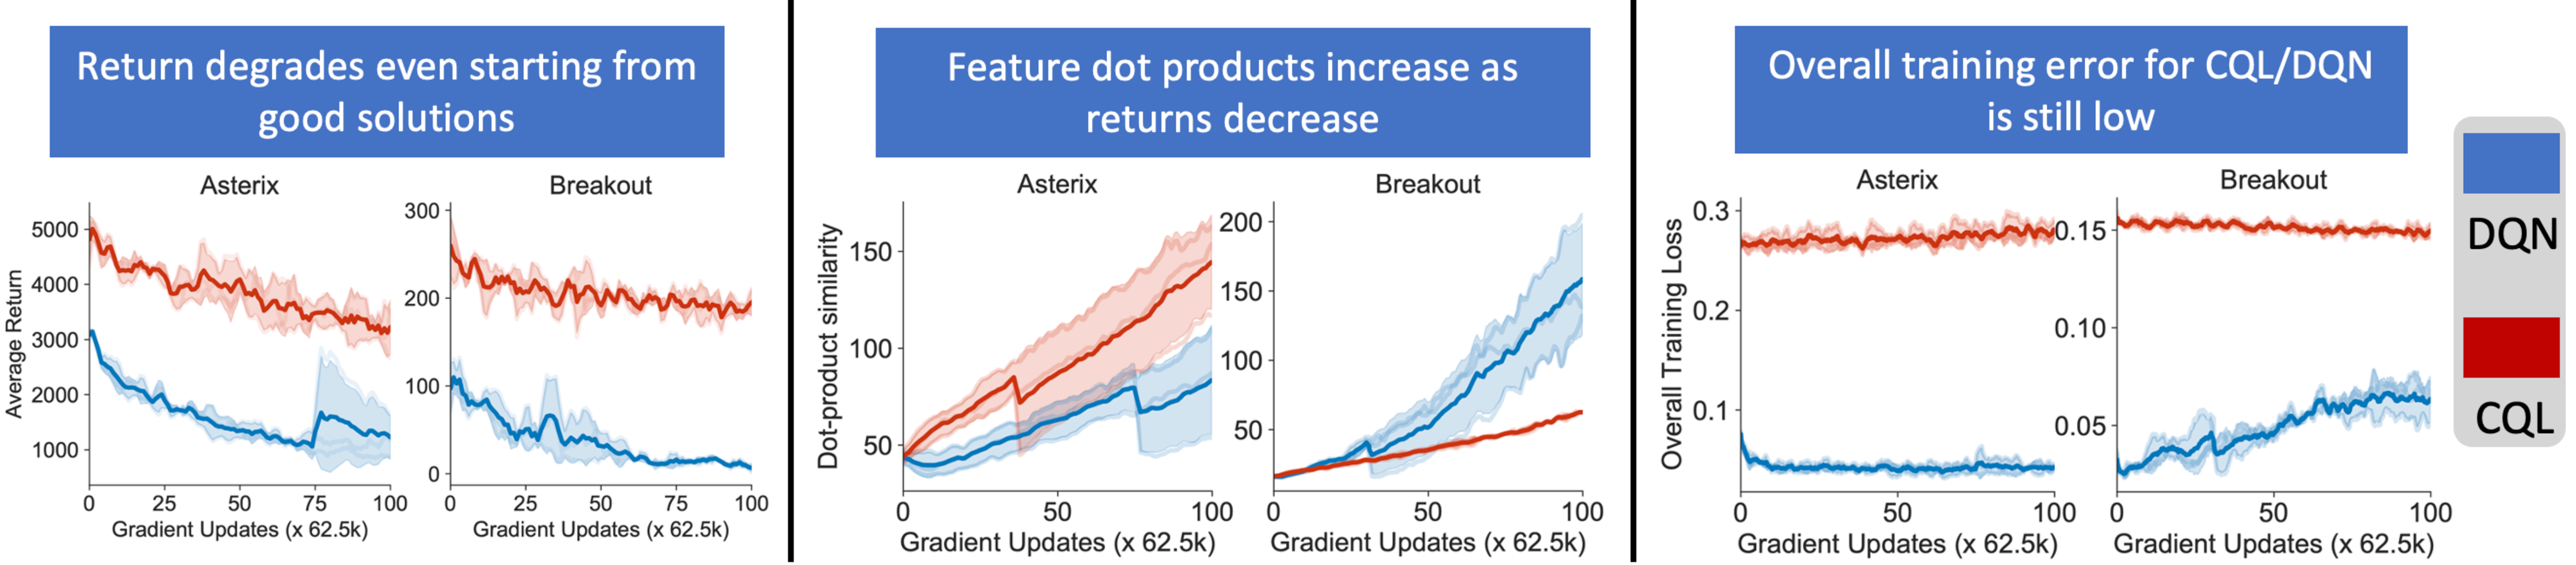
\includegraphics[width=0.99\linewidth]{chapters/dr3/figures_iclr/return_degrades.pdf}
    % 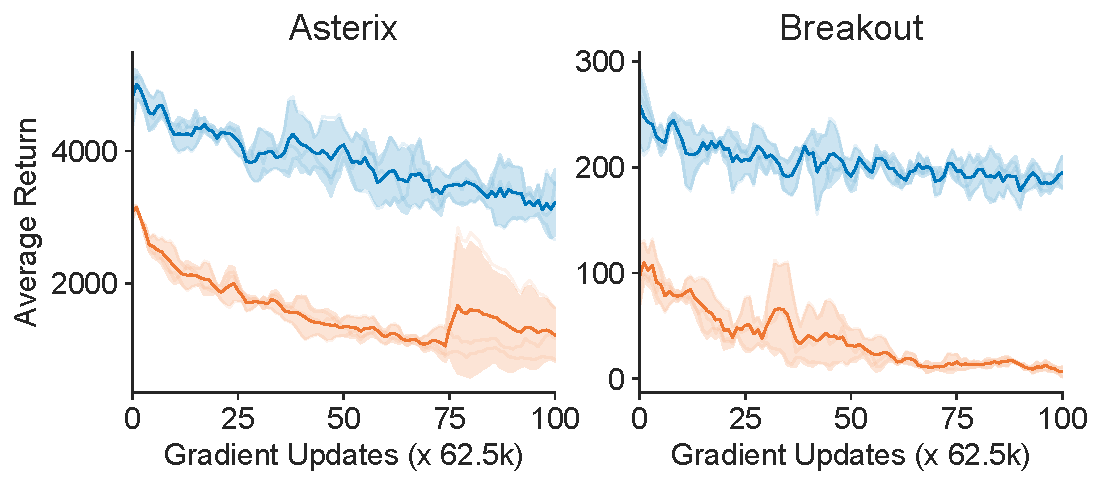
\includegraphics[width=0.49\linewidth]{figures/figure3_neurips_stability_cql_dot_product_both_return.pdf}
    \vspace{-0.3cm}
    \caption{\small{Even when current offline RL algorithms are initialized at a high-performing checkpoint that attains small feature dot products, feature dot products increase with further training and the performance degrades.}}  
    %%SL.7.13: I don't really understand the implication of the last part ("note that the values of the TD error and the overall training loss for either algorithm are generally low and decrease in many cases")
    \label{fig:stability}
    \vspace{-0.3cm}
\end{figure}



\textbf{Why is implicit regularization detrimental to policy performance?}
To answer this question, we present theoretical and empirical evidence that illustrates the adverse effects of this implicit regularizer. Empirically, we ran two algorithms, DQN and CQL, initialized from a high-performing Q-function checkpoint,
%%SL.10.27: This part is going to really throw off some readers. Of course it's not a stable point for TD, because you didn't learn it with TD! Why do we expect the solution found by one method (in this case DR3) to be stable for another method? That doesn't illustrate that TD is bad, just that DR3 changes the fixed point (which it should). But perhaps if you don't want to go into detail about this issue, you could somehow sweep the "obtained using DR3" bit under the rug to avoid distracting the reader?
%%AK: agreed, removed
which attains relatively small feature dot products (i.e., the second term of $R_\mathrm{TD}(\theta)$ is small). Our goal is to see if TD updates starting from such a ``good'' initialization still stay around it or diverge to poorer solutions. Our theoretical analysis in Section~\ref{sec:dr3_theory} would predict that TD learning would destabilize from such a solution, since it would not be a stable fixed point. Indeed, as shown in Figure~\ref{fig:stability}, the policy immediately degrades, and the the dot-product similarities start to increase. This even happens with CQL, which explicitly corrects for distributional shift confounds, implying that the performance drop cannot be directly explained by the typical out-of-distribution action explanations. To investigate the reasons behind this drop, we also measured the training loss function values for these algorithms (i.e., TD error for DQN and TD error + CQL regularizer for CQL) and find in Figure~\ref{fig:stability} that the loss values are generally small for both CQL and DQN. This indicates that the preference to increase dot products is not explained by an inability to minimize TD error. 
%%SL.12.5: I don't understand what "implicit phenomenon" means or how the loss being low indicates this
In Appendix~\ref{app:cql_stability}, we show that this drop in performance when starting from good solutions can be effectively mitigated with our proposed \methodname\ explicit regularizer for both DQN and CQL. Thus we find that not only standard TD learning degrades from a good solution in favor of increasing feature dot products, but keeping small dot products enables these algorithms to remain stable near the good solution.
%%SL.12.5: I slightly tweaked the above sentence, but it can be badly misunderstood as saying that basically our entire evaluation of DR3 has been offloaded into that appendix.

To motivate why co-adapted features can lead to poor performance in TD-learning, we study the convergence of linear TD-learning on co-adapted features. Our theoretical result characterizes a lower bound on the feature dot products in terms of the feature norms for state-action pairs in the dataset $\mathcal{D}$, which if satisfied, will inhibit  convergence: 
\begin{tcolorbox}[colback=blue!6!white,colframe=black,boxsep=0pt,top=-3pt,bottom=2pt]
\vspace{2mm}
\begin{proposition}[TD-learning on co-adapted features]
\label{thm:co_adapted_features_are_bad}
Assume that the features $\Phi = [\phi(\bs, \mathbf{a})]_{\bs, \mathbf{a}}$ are used for linear TD-learning. Then, if 
$$\sum_{\bs, \mathbf{a}, \bs' \in \mathcal{D}} \phi(\bs, \mathbf{a})^\top \phi(\bs', \mathbf{a}') \geq \frac{1}{\gamma} \sum_{\bs, \mathbf{a} \in \mathcal{D}} \phi(\bs, \mathbf{a})^\top \phi(\bs, \mathbf{a}),$$ 
linear TD-learning using features $\Phi$ will not converge. 
\end{proposition}
\end{tcolorbox}
A proof of Proposition~\ref{thm:co_adapted_features_are_bad} is provided in Appendix~\ref{app:new_thm} and it relies on a stability analysis of linear TD. While features change during training for TD-learning with neural networks, and arguably linear TD is a simple model to study consequences of co-adapted features, even in this simple linear setting, Proposition~\ref{thm:co_adapted_features_are_bad} indicates that TD-learning may be non-convergent as a result of co-adaptation.

% \textbf{Comparison to implicit regularization in TD learning with linear function approximation.} Running stochastic gradient descent in overparameterized linear regression finds solutions with the smallest $\ell_2$ norm, which is often regarded as the implicit regularizer. Based on this observation, one might wonder how our derived implicit regularizer relates to minimum norm solutions attained by gradient descent in overparameterized linear TD learning. The implicit regularizer we obtain in  Equation~\ref{eqn:regularizer} would be a constant, independent of the parameter vector $\theta$ for linear TD learning. Thus our regularization specifically captures the effect of SGD on non-linear function approximators, which are absent when studying linear function approximation. 

% \textbf{Takeaways.} We summarize the key takeaways from our theoretical analysis now. \textbf{(1)} \emph{The implicit regularizer at TD fixed points} is shown in Equation~\ref{eqn:regularizer}. The first term corresponds to the regularizer for SGD in supervised learning, while the second term that is unique to TD and leads to an (undesirable) increase in gradient or feature dot products; \textbf{(2)}\emph{Out-of-sample actions exacerbate the implicit regularization effect,} since feature dot products can be easily increased when out-of-sample actions, which do not appear in the dataset, are used to compute Bellman targets; \textbf{(3)} The implicit regularizer in Equation~\ref{eqn:regularizer} is induced via a mechanism unique to non-linear Q-functions, different from overparameterized, linear TD-learning.
% \vspace{-0.15cm}

% \textbf{Theoretically,} we characterize the adverse effects of this implicit regularization by examining the trend in the worst-case error incurred by value-function learning on top of the learned features as feature dot-products increase.


\iffalse
We will first derive the implicit regularization effect induced due to noise in stochastic gradient descent. Following prior work~\citep{blanc2020implicit} in supervised learning, we will model this noise as additive Gaussian noise added to the regression targets. \citet{blanc2020implicit} has identified that in supervised learning, SGD with label noise
%%SL.5.26: is the "label noise" part even significant? almost any supervised learning problem assumes label noise
diverges from a solution $\theta^*$ corresponding to a loss function $L(\theta)$, if and only if it is not a first-order stationary point of:
%%SL.5.26: I found the above sentence pretty hard to parse, can we state this in a simpler way?
\begin{equation*}
    \min_\theta~~ R(\theta) ~~~ \text{s.t.}~~~ L(\theta) = 0,
\end{equation*}
where $R(\theta)$ is an implicit regularizer given by the mean squared L2-norm of the gradient of the learned function with respect to its parameter $\theta$.
%%SL.5.26: add an equation for this
Our goal in this section is to derive the corresponding regularizer for TD-learning, $R_\mathrm{TD}(\theta)$, under similar assumptions, and then analyze its effect on the solution found via TD-learning.  

We first set up the notation. Let $Q_\theta(\bs, \mathbf{a})$ denote the Q-network; for brevity, we will use $\bx$ as shorthand for $(\bs, \mathbf{a})$, such that $\bx := (\bs, \mathbf{a})$ is the input to $Q_\theta$. Given a dataset $\data = \{(\bs_i, \mathbf{a}_i, r_i, \bs'_i)\}_{[n]}$ and following prior work,
%%SL.5.26: add citation
we will assume that the Q-function minimizes  mean-squared TD-error with added label-noise, $\hat{L}(\theta)$, such that \textcolor{red}{George, can we move the label noise to gradient noise?}
\begin{equation*}
%%SL.5.26: reverse the order here, have \hat{L} come first, then \ell
    \ell_\theta(i) = \frac{1}{2} \left(Q_\theta(\bx_i) - \mathrm{StopGrad}\left[r_i + \gamma Q_\theta(\bx'_i) \right] - \epsilon_i \right)^2; ~~~\epsilon_i \sim \mathcal{N}(0, \sigma^2); ~~~ \hat{L}(\theta) := \frac{1}{n}\sum_{i=1}^n \ell_\theta(i),
\end{equation*}
where $\mathrm{StopGrad}$ denotes the stop-gradient operation typically used in TD-learning, $\epsilon_i$ is random Gaussian scalar noise, and $(\bx_i, \bx'_i)$ represent state-action pairs appearing together in a Bellman backup.
%%SL.5.26: make it more explicit what \bx'_i is
TD-learning would then minimize $\hat{L}(\theta)$ via gradient descent. We will assume that $Q_\theta(\bx_i)$,  $\nabla_\theta Q_\theta(\bx_i)$ and $\nabla^2_\theta Q_\theta(\bx_i)$ are all Lipschitz with some coefficients. 


%%SL.5.26: Can we abstract away some of this derivation into a theorem statement and move the derivation to an appendix? This would help to get the paper under the length limit.
To identify the implicit regularizer, we build on the approach of \citet{blanc2020implicit} for supervised learning. We assume that we initialize the parameter $\theta$ to $\theta_0 = \theta^*$, which is an optimal Q-function, satisfying \emph{all} the Bellman consistency equations on all the states in the MDP, not just the states in the dataset.
%%SL.5.26: Do we need to assume that we *initialize* there? Can we just say that we are analyzing the optimum or something? Is this really the assumption that prior work makes?
Now, we will run gradient descent on the loss $\hat{L}(\theta)$ with a sufficiently small learning rate $\eta$, starting from $\theta_0$. This results in the iterates shown below in Equation~\ref{eqn:gradient_descent}. We will then bound the divergence between the $k$-th gradient iterate $\theta_k$ and $\theta^*$, and derive the condition on $\theta^*$ that allows this divergence $||\theta_k - \theta^*||_2$ to be small. This condition will specify the implicit regularizer $R_\mathrm{TD}(\theta^*)$ at a stable optimum $\theta^*$. The gradient descent equation in Equation~\ref{eqn:gradient_descent} can be simplified as shown below in Equations~\ref{eqn:gradient_descent_simplified} and \ref{eqn:grad_descent2}:
\begin{align}
\label{eqn:gradient_descent}
    \theta_{k+1} &:= \theta_k - \eta \nabla_\theta \hat{L}(\theta_k).\\
    \label{eqn:gradient_descent_simplified}
     \theta_{k+1} &= \theta_k - \eta \sum_i \nabla_\theta Q_\theta(\bx_i) \left(Q_\theta(\bx_i) - (r_i + \gamma Q_\theta(\bx'_i)) - \epsilon_i \right)\\
     \label{eqn:grad_descent2}
    \implies \theta_{k+1} &= \theta_k - \eta \underbrace{\sum_{i} \nabla_\theta Q_\theta(\bx_i) \left[Q_\theta(\bx_i) - (r_i + \gamma Q_\theta(\bx'_i)) \right]}_{\text{(a)} := \nabla_\theta L(\theta_k)} + \eta  \underbrace{\sum_i \nabla_\theta Q_\theta(\bx_i) \epsilon_i.}_{\text{(b)} \sim \mathcal{N}(0, \sigma^2 \nabla_\theta Q_\theta \nabla_\theta Q_\theta^\top).}
\end{align}
Note in Equation~\ref{eqn:grad_descent2} that, due to the additive nature of label noise, the parameters $\theta_k$ evolve based on the gradients of the original TD-error loss function \emph{without} noise ($L(\theta)$, term (a)), along with a data-dependent noise (term (b)) sampled from $\mathcal{N}(0, \sigma^2 \nabla Q_\theta \nabla Q_\theta^\top)$. Next, since $\theta_k$ is initialized in the local neighborhood of $\theta^*$, we can rewrite Equation~\ref{eqn:grad_descent2} in terms of $\nabla^2 L := \nabla^2_\theta L(\theta)|_{\theta^*}$, $\nabla^3 L := \nabla^3_\theta L(\theta)|_{\theta^*}$ and $M := \nabla_\theta Q_\theta \nabla_\theta Q_\theta^\top|_{\theta^*}$ by using Taylor expansion around $\theta^*$. Also note that since $\theta^*$ is a global optimum, $\nabla_\theta L(\theta^*) = 0$. Denoting $\nu_k = \theta_k - \theta^*$, we obtain ($\varepsilon_k \sim \mathcal{N}(0, \sigma^2 \nabla Q_\theta \nabla Q_\theta^\top)$):
%%SL.5.26: why are there two sets of parens on that last equation?
\begin{align}
    \label{eqn:\nu_k}
    \theta_{k+1} ~&= \theta_k - \eta \left( \nabla L + \nabla^2 L (\theta_k - \theta^*) + \frac{1}{2} \nabla^3 L (\theta_k - \theta^*, \theta_k - \theta^*) \right) + \varepsilon_k, ~~~~~~\\
    \label{eqn:recursive_v}
    \implies \nu_{k+1} ~&= (I - \eta \nabla^2 L )\nu_k  - \frac{\eta}{2} \nabla^3 L (\nu_k, \nu_k) + \varepsilon_k, ~~~~ \varepsilon_k \sim \mathcal{N}(0, \eta \sigma^2 M).
\end{align}
From Equation~\ref{eqn:recursive_v} we can make a few observations. First, the distance between $\theta_k$ and $\theta^*$, $||\nu_k||_2$ decreases at a rate proportional to $(I - \eta \nabla^2 L)$. $\nabla^2 L$ only spans certain directions due to the overparameterized nature of the landscape. Thus $\nu_k$ will not contract on along every direction, and the noise $\varepsilon_k$ in each iteration can compound through powers of $(I - \eta \nabla^2 L)$ leading to an increased in the value of $\nu_{k}$,
%%SL.5.26: presumably it makes it increase under some conditions on that matrix?
thus making $\theta_k$ diverge from $\theta^*$. However, if the starting $\theta^*$ is such that the third derivative $\nabla^3 L (\nu_k, \nu_k)$ can compensate for any potential increase in the value of $\nu_k$, then $\nu_{k} \rightarrow 0$ as $k \rightarrow \infty$. Theorem~\ref{thm:implicit_noise_reg} formalizes this to obtain an expression for the resulting implicit regularizer. A proof for Theorem~\ref{thm:implicit_noise_reg} can be found in Appendix ??.
\begin{theorem}[Informal, Implicit regularization at optimal TD-solutions]
\label{thm:implicit_noise_reg}
Assuming notations
%%SL.5.26: "Assuming notations" seems like a weird phrase
and conditions of label-noise gradient descent on TD error discussed so far, a global minimizer of TD error $\theta^*$ on the dataset $\mathcal{D}$ is a stable optimum if and only if it minimizes implicit regularizer $R_\mathrm{TD}(\theta)$ given by:
\begin{equation}
\label{eqn:regularizer}
    R_\mathrm{TD}(\theta) = \mathrm{tr} \left(\sum_{i=1}^n \nabla_\theta Q_\theta(\bx_i) \left( \nabla_\theta Q_\theta(\bx_i) - \gamma \nabla_\theta Q_\theta(\bx'_i) \right)^\top \right).
\end{equation}
\end{theorem}
\textbf{Interpretation of Theorem~\ref{thm:implicit_noise_reg}.} Theorem~\ref{thm:implicit_noise_reg} indicates that out of all possible global minimizers $\theta^*$ of the TD error
%%SL.5.26: this is a fairly basic point, but I think when we introduce the notion of implicit regularization earlier, it might help to expand on what this "out of all possible minimizers" thing means. E.g., something like this: When training overparameterized functions, such as deep networks, multiple different parameter vectors $\theta$ will minimize $L(\theta)$. But not all of these minimizers will generalize equally well. \citet{someone} proposes that the minimizer found via SGD will satisfy the following constrained optimization problem: [stuff], where $R(\theta)$ is an \emph{implicit} regularizer that arises from the structure of SGD with overparameterized models. Intuitively, $R(\theta)$ causes SGD to prefer simpler (and therefore more generalizable) solutions, even when we might otherwise expect overparameterized models to be liable to overfit. This model has been put forward as one explanation for the effective generalization of overparameterized deep networks~\citep{stuff}. [this could go at the top of Sec 3.2.1 for example]
on the training dataset, gradient descent with label noise will only stabilize at a minimizer of $R_\mathrm{TD}(\theta)$. $R_\mathrm{TD}$ consists of two types of terms: positive terms equal to gradient norms, $\sum_i ||\nabla_\theta Q_\theta(\bx_i)||^2_2$, and additional negative terms equal to the expected dot-product of gradients at consecutive states, $\sum_\theta Q_\theta(\bx_i)^\top \nabla_\theta Q_\theta(\bx'_i)$.
%%SL.5.26: Is it completely obvious where these come from? I realize this is just algebra, but we could spoon-feed it to the reader more by writing out the distributed equation so that these terms actually show up.
If all state-action pairs $\bx'_i$ appearing on the right-hand-side of the Bellman update also appear in the dataset $\mathcal{D}$, as in the case of SARSA (Figure~\ref{fig:dot_products}), they would also contribute to the gradient norm term, and the value of $R_\mathrm{TD}$ will be bounded below.  We can show that in this case the optimal $\theta^*$ would effectively minimize $(1 - \gamma) \sum_i ||\nabla_\theta Q_\theta(\bx_i)||_2^2$.
%%SL.5.26: can we make these statements a bit more formal? e.g., have a corollary or something for the special case where all x' are in the dataset, and another one for the case where that is not true?
This corresponds to a regularizer one would obtain when training the Q-network via pure supervised learning~\citep{blanc2020implicit}, indicating that SARSA is regularized in similar ways as supervised regression. 
%%AK: is there consensus on this aspect?

%%AK: I am sure the para below doesnt have a great flow. If someone has any suggestions to make it more dramatic, it will be great -- this is the key RL explanation part of this math.
On the other hand, if a state-action pair $\bx'_i$ only appears on the right-hand-side of the backup, \ie, $(\bs', \mathbf{a}')$ correspond to out-of-sample state-action pairs,
%%SL.5.26: remind the reader why this would be the case, like this: However, the regularizer behaves very differently when some state-action pairs $\bx'_i$ only appear on the right-hand-side of the backup. This happens with any algorithm where $\mathbf{a}'$ is not the dataset action, which is the case for all actor-critic and Q-learning algorithms that compute target values by selecting $\mathbf{a}'$ according to the current policy. Note that $(\bs',\mathbf{a}')$ does not need to be \emph{out-of-distribution}, merely \emph{out-of-sample}, and hence this would even be the case when evaluating $\pi_\beta(\mathbf{a}'|\bs')$ with samples from $\pi_\beta(\mathbf{a}'|\bs')$ for the target value actions.
then the implicit regularizer, $R_\mathrm{TD}(\theta)$ is minimized only at solutions $\theta^*$ for which gradients at $\bx_i$ and the corresponding $\bx'_i$ are very similar in terms of dot-product.
%%SL.5.26: some pretty informal statements here, can we summarize this more precisely in a formal corollary?
This is the co-adaptation phenomenon observed in Section~\ref{sec:analysis}: gradients at out-of-sample state-action pairs $\bx'_i$ are extremely similar to the gradients at $\bx_i$ at the resulting optimum.
%%SL.5.26: gradients are similar? or features are similar?
Section~\ref{sec:analysis} instead demonstrated the co-adaptation phenomenon for penultimate layer features, which are also the gradients with respect to the parameters of the last layer, since these values are cheap to compute.
%%SL.5.26: put the above in a footnote, phrase like this: One discrepancy is that Section~\ref{sec:analysis} analyzes dot products between the last-layer features, whereas this derivation focuses on dot products between gradients. Note, however, that the last-layer features are the gradients of the weights in the last layer. [maybe allude to some NTK stuff?]. Alternatively, given that you use "gradients" and "features" interchangeably below, you could also put some discussion like this in the main text, but earlier: Note that this regularizer concerns the \emph{gradients} of the model. However, regularization of gradients and regularization of features are closely related~\citep{something} -- for example, the gradients of the last-layer weights are equal to the penultimate layer features for networks with linear readout layers.
Thus, we have shown that stochastic gradient descent on the TD-error tends to stabilize only at solutions that exhibit highly co-adapted features between out-of-sample points used for the backup and the points in the dataset. \textcolor{red}{also add when it will diverge; tr(...) cant be < 0, else we wont contract.}
\fi


\iffalse
\subsubsection{Implicit Regularization of Neural Network Architectures}
%%SL.5.26: Change the title -- the point is not that it's architecture specific, but that it is focused on overparameterization and min norm.

In the previous section, we showed, that agnostic of the neural network architecture, implicit regularization arising out of the stochasticity in SGD produces Q-functions with highly co-adapted features. In this section, we analyze a different kind of implicit regularization originating from the inductive bias and invariance of the neural network architecture.
%%SL.5.26: This seems like a really strange way to "sell" this analysis -- it's basically saying that before we analyzed the general case, now we'll make some more (unrealistic) assumptions and show that the results still hold under these additional (unrealistic) assumptions. That's a very strange statement. The fact that this analysis is architecture-specific is not really a plus. Can we come up with a better way to motivate why we have this analysis? A reasonable way to go could be something like: In this section, we will show that a similarly deleterious implicit regularization effect in TD-learning can be derived from a very different model of implicit regularization with overparameterized deep networks, based on minimum norm solutions. [and then at the end of this subsection, you can conclude with something like: We've shown that two very different models of implicit regularization in deep nets proposed in prior work~\citep{} both lead to the same conclusion in the TD-learning setting: the very same implicit regularization effects that promote effective generalization in supervised deep learning lead to learning of features that can fail to distinguish between successive state-action tuples in the TD-learning setting.]
For this analysis, we study a 2-layer wide ReLU network using ideas from prior works~\citep{blanc2020implicit,savarese2019infinite,wei2019regularization}.
%%SL.5.26: can we rephrase the above sentence and talk about how we adopt a similar model of implicit regularization as prior work?
For simplicity, we assume that the input space of the Q-function is 1-dimensional, which can be attained by mapping state-action pairs $(\bs_i, \mathbf{a}_i)$ to a one-dimensional representation $\bx_i \in \mathbb{R}$, though our argument can potentially be generalized to higher-dimensional inputs analogous to \citet{}.
%%SL.5.26: Whoa, that seems like a crazy assumption. Is that really how prior work does it?? I mean, I can see how this can be made to work, but it's an enormous leap.
%%AK: cite the savarese paper 2 from 2019 that uses radon transform

To begin, we define a canonical 2-layer ReLU network with 1D inputs: $Q_\theta(\bx_i) = \sum_i \bw_i \sigma(\mathbf{a}_i \bx_i + \bb_i) + \bd_i$, where $\sigma(\cdot) = \max(\cdot, 0)$ is the ReLU function. It is well known~\citep{wei2019regularization,savarese2019infinite} that minimizing $L(\theta) = \sum_i (Q_\theta(\bx_i) - y_i)^2$ for input-output pairs $(\bx_i, y_i)$ on a 2-layer ReLU network of sufficient width produces a solution that satisfies the following optimization (left):
%%AK: The para above is not talking about TD-learning but optimizations already use TD, so I need to fix that.
%%SL.5.26: yeah, this is an issue -- above says y, below says r + gamma*Q
\begin{equation}
\begin{aligned}
    &\text{\textbf{Neural Network parameterization}} \\
    \min_{\bw, \mathbf{a}, \bb, \bd}~~& ||\bw||_1 \\
    \text{s.t.}~&~ \forall~ \bx_i \in \mathcal{D},~~ Q_\theta(\bx_i) = r_i + \gamma \mathbf{a}r{Q}_\theta(\bx'_i) 
    \label{eqn:relu_nets}
\end{aligned}
\;~~ \vline\;
\begin{aligned}
    &\text{\textbf{Function space parameterization}} \\
    ~~~\min_{Q}~~& \int_{-\infty}^{\infty} |Q''(\bx)| d \bx \\
    \text{s.t.}~~&~ \forall \bx_i \in \mathcal{D}, ~~ Q(\bx_i) = r_i + \gamma \mathbf{a}r{Q}(\bx'_i).
\end{aligned}
\end{equation}
The optimization on the left can be converted to a function space parameterization (Equation~\ref{eqn:relu_nets}, right) that minimizes the second-derivative of the function $Q''(\bx)$ w.r.t. the input $\bx \in \mathbb{R}$ while fitting the data. This amounts to fitting the smoothest possible function that attains zero Bellman error.
%%SL.5.26: Let's just introduced the supervised model *first*, and only then talk about Bellman error, otherwise we are throwing more at the reader than they can reasonably handle.
In supervised learning this gives rise to a piecewise linear function with kinks at the points from the dataset, $\bx_i \in \mathcal{D}$ (Theorem 3.1 in \citet{savarese2019infinite}). In our case, we are interested in answering the following question: Among all solutions with zero Bellman error on the training data, do co-adapted solutions attain maximum smoothness? 
%%SL.5.26: That doesn't seem like the right way to pose the question, because "maximum smoothness" is a vague and imprecise term. Let's rather refer to the formal statement of the objective.

To answer this question, we first set up some notation. Let $(\bx_i, \bx'_i)$ be the representations of state-action tuples that appear together in a Bellman update.
%%SL.5.26: already defined this
Without loss of generality, let $\{\bx_i\}_{[n]} \in \mathcal{D}$ be ordered as $\bx_1 < \bx_2 < \cdots < \bx_N$. We further make a locality assumption on the consecutive tuples:
\begin{assumption}[State-action pairs on two sides of a Bellman backup are close to each other]
\label{assumption:state_next_state_are_close}
If $(\bx_i, \bx'_i)$ appear on the two sides of the Bellman equation, and if $\bx_{i-1}$ and $\bx_{i+1}$ be the left and right neighbors of $\bx_i$ observed in $\mathcal{D}$, then, we assume $|\bx_i - \bx'_i| \leq \min \left(|\bx_i - \bx_{i-1}|, |\bx_{i+1} - \bx_i| \right)$. 
\end{assumption}
Assumption~\ref{assumption:state_next_state_are_close} encodes the notion that the next state,
%%SL.5.26: Don't overload terminology, you're using "state" to mean two different things. This will be perceived as (intentionally) deceptive, because the consecutive actions are *not* similar.
$\bx'_i$, is closer to the current state $\bx_i$ compared to the neighbors of $\bx_i$ found in the dataset. This is reasonable to assume in practice, where states and next states generally do not differ from each other by a huge amount, often changing by a few pixels.
%%SL.5.26: I disagree with the above statement -- why the heck would \bx'_i be closer to \bx_i than \bx_{i+1}? Presumably the next action of pi_beta is at least as close to the current action of pi_beta than the next action of pi. Maybe you mis-stated something above and intended to write something else? But as written this just doesn't seem plausible.
%%AK: is there a better, simpler assumption? And can I cite something to say that the states- next states are closeby?
Under Assumption~\ref{assumption:state_next_state_are_close}, we show the following result:
%%AK: refine theorem statement and verify edge cases once (a lot of the edge cases are measure zero, so maybe just almost surely will eliminate time?)
\begin{theorem}[Informal, ReLU networks attain additional kinks
%%SL.5.26: let's avoid informal statements in theorems ("kinks")
and learn incorrect Q-values]
\label{thm:relu_nets_kinks}
Assuming~\ref{assumption:state_next_state_are_close} and other notation from this section, the optimal solution for Equation~\ref{eqn:relu_nets} (right) consists of kinks
%%SL.5.26: that doesn't seem like a precise theorem statement...
at $\mathcal{D} \cup \{\bx'_1, \cdots, \bx'_n\}$. Moreover, the Q-values at any $\bx_j$ for which $\bx'_j \notin \mathcal{D}$ will be incorrect.
%%AK: TODO: refine the theorem to make it more formal
\end{theorem}
%%AK: TODO; also add SARSA discussion?
When fitting supervised targets to a deep ReLU network, the resulting solution is a piecewise linear function, with pieces intersecting only at the datapoints $\bx_1, \cdots, \bx_n$. On the other hand, Theorem~\ref{thm:relu_nets_kinks} shows that the optimal solution that satisfies Bellman equations will have additional kinks on out-of-sample state-action tuples used for the backup, i.e., $\{\bx'_1, \cdots, \bx'_n\} \mathbf{a}ckslash \mathcal{D}$. These kinks will alter the values learned at several other state-action pairs, while still satisfying Bellman constraints on the training data and being more smooth as measured by the integral of the second derivative of the function. This is a form of co-adaptation: implicit regularization towards smooth functions in a ReLU network makes predictions at $\bx$ and $\bx'$ coupled together so as to maximize smoothness. Having seen that implicit regularization stemming from a variety of factors including noisy updates and neural network architectures when combined with TD error and gradient descent and its direct relationship with feature co-adaptation, the next section aims to devise an explicit regularizer that can tackle these adverse effects of implicit regularization.   
\fi


\iffalse
\subsection{Consequences of Feature Co-Adaptation in TD-Learning}
Having seen that TD-learning co-adapts features at unseen actions to features at state-action tuples in the dataset, we now study its consequences. We will show that this co-adaptation can prevent learning high-frequency information in the Q-function crucial for control and destabalize learning, even when initialized in the vicinity of a good solution.

\begin{wrapfigure}{r}{0.4\textwidth}
    \centering
    \vspace{-22pt}
    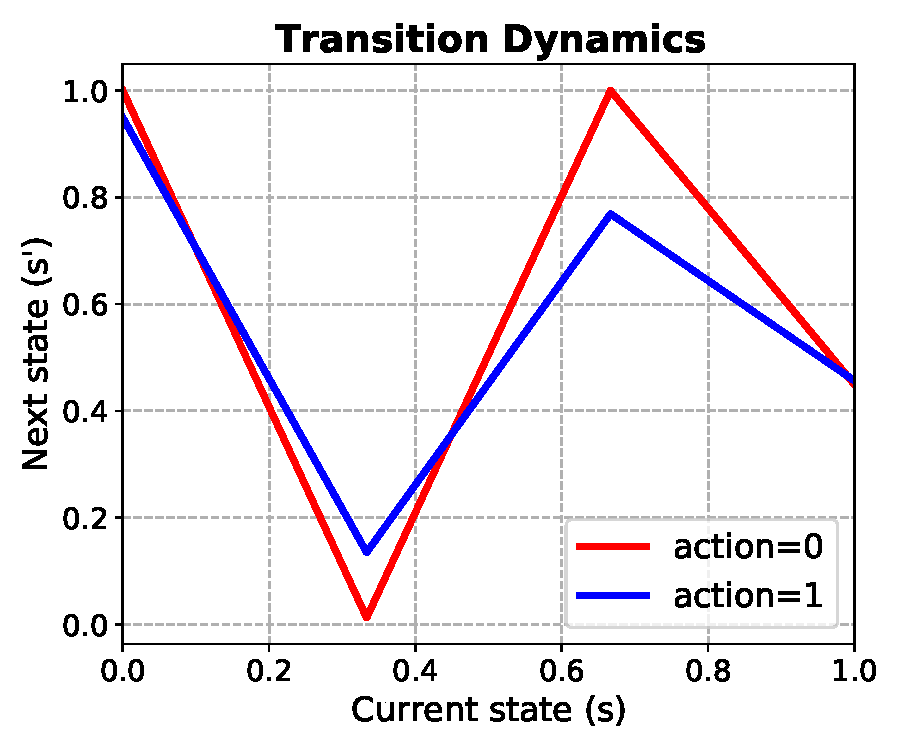
\includegraphics[width=0.48\linewidth]{chapters/dr3/section3_figs/dynamics.pdf}
    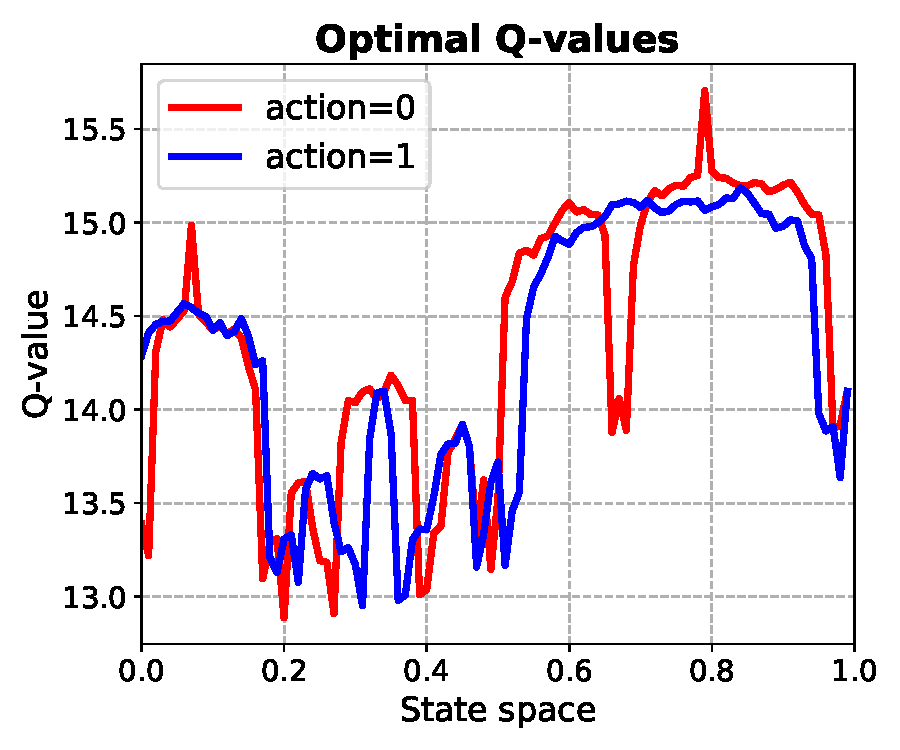
\includegraphics[width=0.48\linewidth]{chapters/dr3/section3_figs/optimal_q.pdf}
    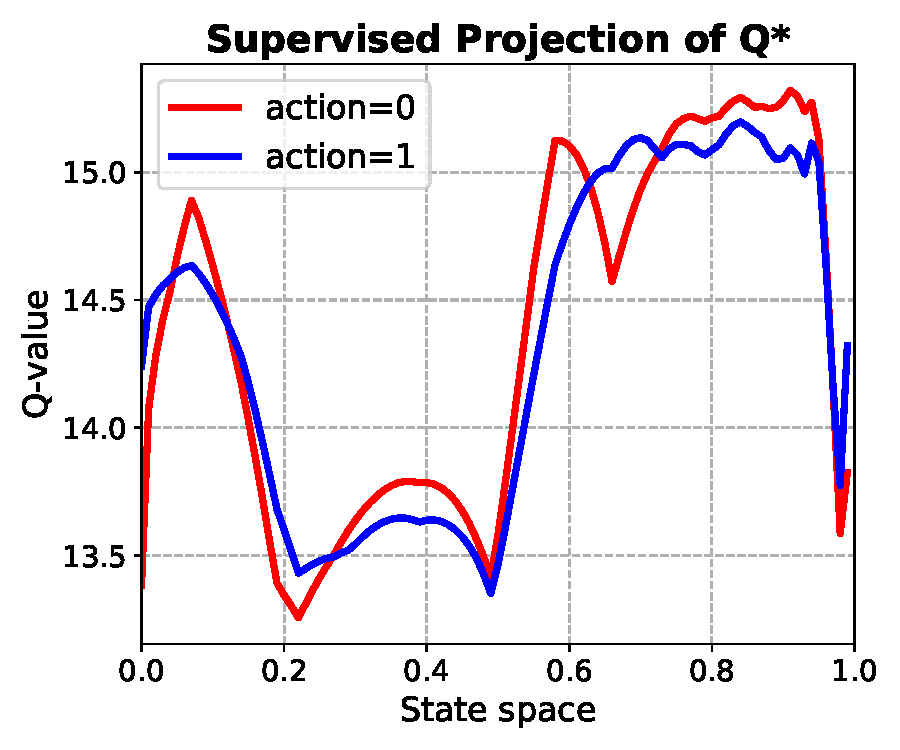
\includegraphics[width=0.48\linewidth]{chapters/dr3/section3_figs/supervised_q.pdf}
    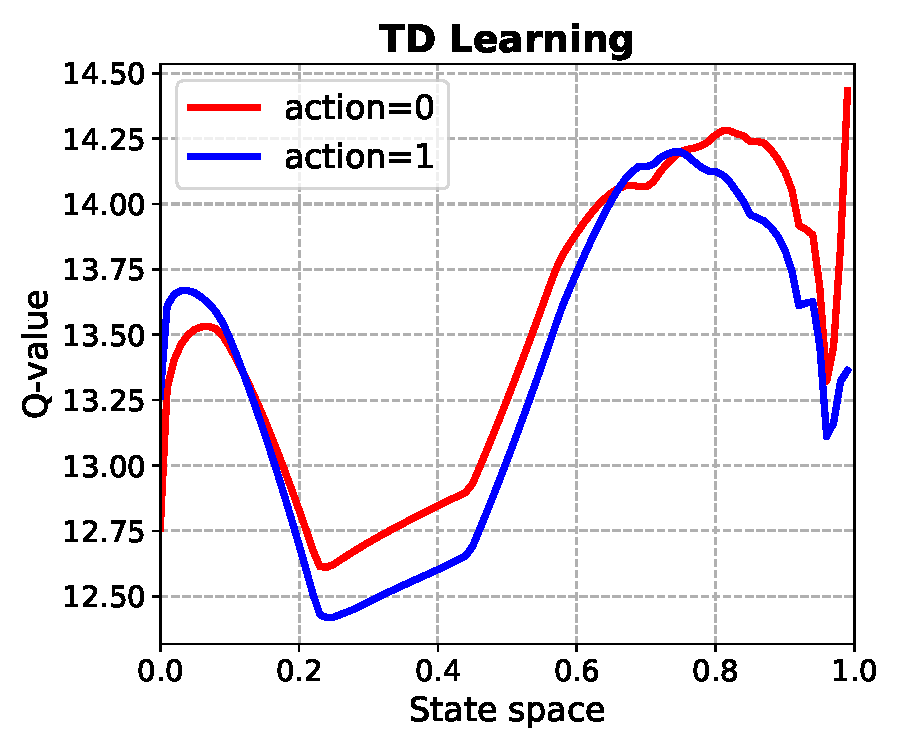
\includegraphics[width=0.48\linewidth]{chapters/dr3/section3_figs/td_learning.pdf}
    \vspace{-0.21cm}
    \caption{\small{\textbf{TD-learning fails to represent high frequency changes in Q-functions much more than supervised learning.} On the 1D MDP (dynamics, top-left), TD learning ignores the high-frequency components of the Q-function leading to worse action selection compared to supervised regression.}} 
    \label{fig:1d_mdp}
    \vspace{-0.6cm}
\end{wrapfigure}
%%AK: Tengyu had an interesting suggestion here: represent the action choices of each function via a shaded interval on the the number line, using blue for a_0 and red for a_1. The number of switches will determine the complexity of the Q-function, and this will show that TD has 4 switches, supervised has 8 and actual has 12 or 13 switches.
\textbf{Inability to model high-frequency components of Q-function.} Prior work has noted that Q-functions can be highly non-smooth even when reward functions and dynamics are relatively simple~\citep{dong2020expressivity}.
%%AK: does gamma models also note something related to complexity of Q vs reward via the discount profile stuff?
Would feature co-adaptation lead the Q-function to ignore certain high-frequency components in the objective?
As a didactic example of this phenomenon, we utilize a 2-action MDP with a 1-D state space $\mathcal{S} \in [0, 1]$ from~\citep{dong2020expressivity}. This MDP exhibits a piecewise linear dynamics (Fig.~\ref{fig:1d_mdp}, top-left) and an identity reward function $r(\bs, \mathbf{a}) = \bs$ with two actions $\mathbf{a} \in \{0, 1\}$. The optimal Q-function exhibits high-frequency changes (Fig.~\ref{fig:1d_mdp}, top-right). We find that running Q-learning (Fig.~\ref{fig:1d_mdp}, bottom-right)
attains Q-functions that completely ignore these high-frequency changes. This often makes the resulting policy choose the worse action of the two possible actions. On the contrary, a supervised projection (Fig.~\ref{fig:1d_mdp}, bottom-left) of the Q-function does capture many of these high frequency shifts in the Q-function. To formalize this didactic example, we prove the following result showing that high-frequency components of the Q-function are not modelled as a direct consequence of Theorem~\ref{thm:aliasing_exists}. The proof and a complete statement for Theorem~\ref{thm:num_pieces} can be found in Appendix ??.

%%AK: this will have some conditions on dynamics too, maybe we mention that as a detail in the appendix? But if it is unclear, maybe we should add it here, and explain it here...
\begin{theorem}[Informal]
Assume that the state-space $\mathcal{S}$ of the MDP is given by the 1-D number line, and that the groundtruth Q-function is (approximately) piecewise linear in the state $s$ with $N^*$ pieces. Denote the (approximate) number of linear pieces in a learned infinite-capacity ReLU Q-network via direct supervised regression as $N_{\mathrm{Sup}}$ and via TD-learning as $N_{\mathrm{TD}}$. Then: $N_{\mathrm{TD}} \leq N_{\mathrm{Sup}} \leq N^*$.     
\label{thm:num_pieces}
\end{theorem}
%%AK: In the proof of this theorem, we show this for approximate number of pieces, which is the integral of the second derivative of the function w.rt.t the input over the input space, but I think going into details would just hurt understanding here.

%%AK: I am a little unsure about the following part, in the sense if we should have it or not? This might seem obvious to some extent? 
% \textbf{Severe co-adaptation renders distributional shift corrections ineffective.} To test whether offline RL corrections alleviate feature co-adaptation, we performed a controlled experiment -- we constrained offline RL regularizers to only control the last linear layer of the Q-network, whereas bootstrapping was allowed to train the entire network. While we might expect that offline RL methods may still be effective by adapting the last weight layer to the features, contrary to this expectation, as shown in Figure ??, we find that all such variants (denoted as CQL($\phi$)) perform extremely poorly compared to the complete offline RL method. Further note the inability to minimize the regularizer corresponding to distributional shift and an increased dot-product similarity, $\Delta(\bs, \mathbf{a}, \bs', \mathbf{a}')$. This indicates that feature co-adaptation can lead to failure of offline RL methods. \textcolor{red}{add new figure for this}
%%AK: If we do keep this, maybe we should also add some line to justify why offline RL methods are still sensitive -- this is because they are not exactly doing SARSA?

\textbf{Lack of stability near ``good'' Q-function solutions.}
%%SL.5.22: instead of using a vague term like "good" with scare quotes, can we just say optimal? And what does "lack of stability" mean? Maybe just state it directly: Implicit regularization can prevent convergence, even when initializing at an optimal solution. [or something like that]
Finally, we study if co-adaptation of features cause the TD-learning process to diverge away, even when initialized favorably in the vicinity of a good Q-function (e.g., one obtained via supervised regression to MC returns or one obtained via online RL). Running Q-learning from such a favorable initialization eventually produces solutions that perform poorly as shown in Figure ?? below. Moreover, \textcolor{red}{say something about ranks here}. Indeed, in accordance with Theorem~\ref{thm:aliasing_exists}, the feature co-adaption phenomenon drives learning towards solutions with lower $\srank(\bM_{\mathrm{TD}}(\phi))$ values, giving rise to poor performance. \textcolor{red}{add figure, theorem}      
\fi

%%SL.5.17: what are Bellman constraints?
% are only enforced approximately (i.e., when the TD error
% %%SL.5.17: was the TD error ever defined?
% is not exactly 0), the implicit regularization towards minimum $||\bw||_2$ norm solutions will lead to the Q-function ignoring high-frequency components. That is, if the true Q-function changes dramatically from one state to the next, low TD-error solutions will fail to represent these changes.
%%SL.5.17: I don't see why the above theorem indicates that this is true
%%AK: add a worst-case theorem as discussed with George today?
%%SL.5.17: maybe we should put this didactic example into a separate \paragraph{} with more setup, instead of presenting this as a kind of footnote -- as-is, I think many people will not really understand it


%%AK: Check if we can take this paper's "peicewise linear theory" and convert it to a policy improvement bound differentiating between TD and supervised, as opposed to just fitting Q*-values?

% \subsection{Consequences of Overly Regularized Representations in TD Learning}
% Having seen aliasing of features on state-action tuples used for bootstrapping emerge as one pathological consequence of overly regularized representations in TD-learning compared to supervised learning, we next ask the following question we study the impact of over-regularization have on the performance of TD-learning. In particular, we ask: do TD-learning algorithms find generalizing and stable optima? To answer these questions, we consider a simple scenario where learning is initialized from a 


% \textbf{Abstract model.} Our abstract model captures feature learning as making a discrete selection among $K$ different feature vector candidates, $\{\Phi_1, \Phi_2, \cdots, \Phi_K\}$, $\Phi_i \in \mathbb{R}^{|\data|\times d}$,
%%SL.5.13: It would be way easier to understand if we could get continuous domains, and then just frame this as an optimization over \Phi (i.e., optimization over \Phi corresponds to selecting the best \Phi \in [some set]), that way we don't have to have this "discrete selection" business and could just say that it's part of the optimization process.
% and then training a linear layer $\bw \in \mathbb{R}^{d}$ to obtain the Q-function.
%%SL.5.13: One way you could phrase is this: Our abstract model of the learning process separates the neural network into two parts: a representation $\Phi$ and a weight vector $\bw \in ...$, such that the full model is given by $\Phi(..)^T \bw$ (i.e., $\bw$ corresponds to the last linear layer). The learning process is framed as a \emph{bilevel} optimization problem, where the weights $\bw$ are chosen subject to a constraint that the learning process chooses the optimal features $\Phi \in [set]$ for $\bw$ (or something like that)
% To mimic the overparameterized nature of neural networks, we assume that we operate in the overparameterized regime with $n < d$.
%%SL.5.13: This is kind of weird -- usually the last layer features are not that high dimensional, but the model parameters are. Are you sure we shouldn't look for some way to "NTK-ify" this? Perhaps a better way to frame this is that we are in the NTK regime where the choice of Phi corresponds to the choice of NTK (i.e., it's not fixed, as is more common in this analysis), while bw corresponds to the neural net parameters? That would justify the overparameterized regime and make this less weird.
% Assume that the initial value of the weight vector $\bw^{(0)} = 0$. We then write out the minimum-norm optimization problem shown below in Equation~\ref{eqn:min_norm} that attains the same solution as the optimal solution found by minimizing training TD error in this model, and characterize the properties of features $\Phi_K^*$ that are selected to obtain the minimum-norm solution. \textcolor{red}{more assumptions?}     
%%SL.5.13: It won't be clear to some people what min-norm has to do with neural net training, can you cite something to justify this?
% \begin{align}
%     \min_{\bw, \boldm_i \in \{0^d, 1^d \}}~~& ||\bw||_2^2 \nonumber\\
%     \text{s.t.}~~&~ \mathbf{a}r{\Phi}^\top \mathbf{a}r{\Phi} \bw = \mathbf{a}r{\Phi}^\top R + \gamma \mathbf{a}r{\Phi}^\top P^\pi \mathbf{a}r{\Phi} \bw, ~~ \mathbf{a}r{\Phi} = \left[\Phi_1, \cdots, \Phi_k\right] \otimes [\boldm_1, \cdots, \boldm_K]
% \label{eqn:min_norm}
% \end{align}
%%SL.5.13: ouch, this \bm_i is... difficult to parse
% Our first result characterizes the feature representation $\mathbf{a}r{\Phi}$ -- equal to one of $\Phi_i$ selected based on the learned masks $\bm_i$ -- that satisfies the Bellman consistency condition but also minimize the implicit regularizer, $||\bw||_2^2$,
% %%SL.5.13: where does this implicit regularizer come from?
% and use this to depict the existence of this phenomenon.


\iffalse

\section{Representation Regularization in Offline Q-Learning}
\label{sec:problem}
%%SL.5.13: See my comment on the title about "excessive" (maybe we call it Implicit Over-Regularization?). That said, this again sounds *extremely* similar to IUP, to the point where the section title alone could lead many readers to suspect this is just a direct copy of the IUP paper.
%%AK: yeah I agree. I am a little unsure what to call it, besides maybe admitting that this is similar IUP in high-level motivation but not low-level technical details. Do you think that's doable? My rationale was that right now readers might have the impression that we are trying to do something like IUP but also trying to distinguish it from IUP, without making clear what our contribution is and what's already there. Perhaps just saying something like "Fine-grained analysis" or something that explicitly quantifies the extent of this contribution is different? Avoiding that might just create questions. What do you think?
%%AK: the title sounds lika having a good connotation, is there a bad word for "regularization" that is not just "over-regularization" or "aliasing"?

% In this section, we study the mechanism by which implicit regularization effects are induced in offline Q-learning, and discuss how these effects can lead to pathological issues such as overly aliased representations and convergence to poor solutions. These aliasing properties exist even when learning is initialized from good solutions that do not exhibit this aliasing, and can make the learning eventually diverge. We first provide an empirical analysis of this phenomenon and then theoretically formalize these observations in a simple abstract model of learning dynamics of Q-learning.
Offline RL algorithms discussed previously are unstable and suffer from hyperparameter tuning challenges. A simple choice such as the number of training steps can be game-changing -- too few gradient steps will of course give rise to underfitted Q-functions, but perhaps surprisingly, too many gradient steps also lead to poor performance (Figure~\ref{fig:atari_5_percent}, Figure 2 in \citep{kumar2021implicit}). This phenomenon resembles statistical overfitting at first, however, it is actually underfitting caused due to excessive representational regularization of training deep networks with TD error that manifests as aliased features. While this issue has been broadly noted in previous work~\citep{kumar2021implicit}, in this section we will provide a fine-grained analysis of this phenomenon first empirically and then theoretically. In Section~\ref{sec:method}, we will then discuss a simple regularization scheme that can mitigate this issue. \textcolor{red}{TODO}  
%%SL.5.13: Maybe a somewhat more forceful lead-in could look like this:
% While the offline RL algorithms discussed in the previous section mitigate the worst challenges of offline RL~\citep{bear}, effectively using such methods in practice still requires extensive hyperparameter tuning. A particularly delicate choice is the number of gradient steps to take on the offline dataset -- too few gradient steps obviously produce underfitted, suboptimal value functions. But surprisingly, too many gradient steps also often result in poor performance, as illustrated in Figure ??. What is the reason for this performance collapse? While this phenomenon initially resembles overfitting, it is in fact an instance of \emph{underfitting}: although deep networks trained with SGD should provide a very good fit in standard supervised settings, we will argue that training with TD backups introduces a pathological over-regularization effect, induces excessive aliasing, and greatly constrains the expressive power of the resulting features. We first analyze this empirically, and then present a theoretical analysis. In Section ??, we will discuss how a simple regularization scheme can mitigate this issue.
%%AK: I havent added this fully, and instead cited IUP for the basic "noting" of this phenomenon and then said that we provide finegrained analysis of it. But I can change it. 

\iffalse
\subsection{Empirical Analysis}
\label{sec:empirical_analysis}
\begin{wrapfigure}{r}{0.49\textwidth}
    \vspace{-47pt}
    \centering
    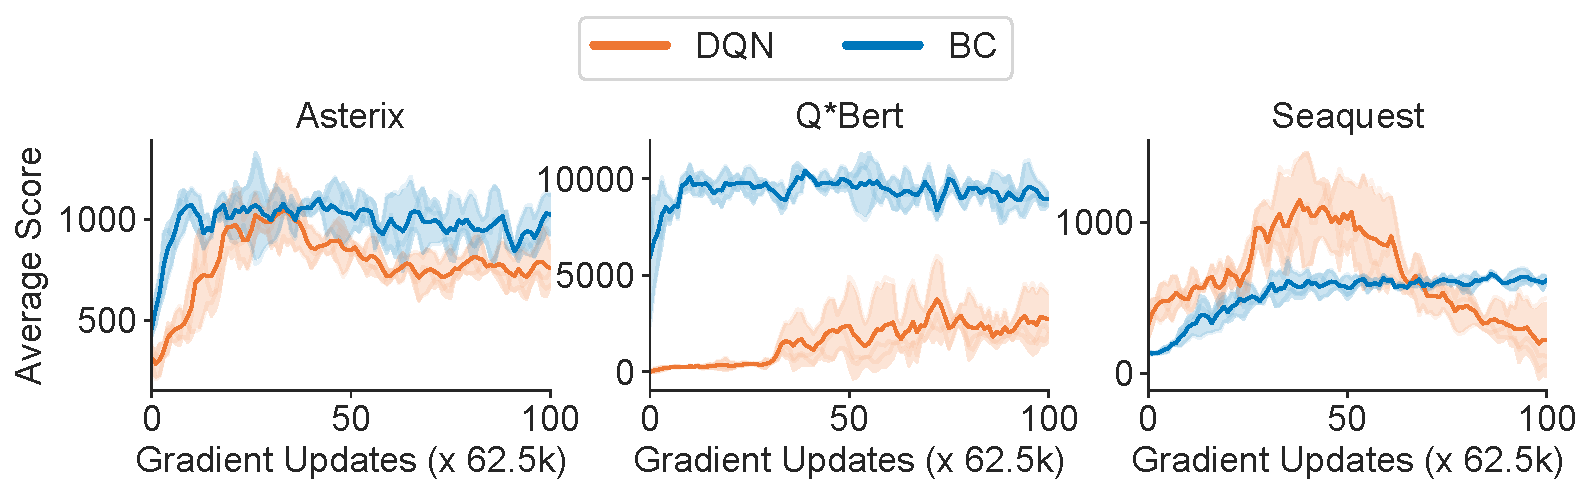
\includegraphics[width=\linewidth]{chapters/dr3/atari/perf_3_games.pdf}
    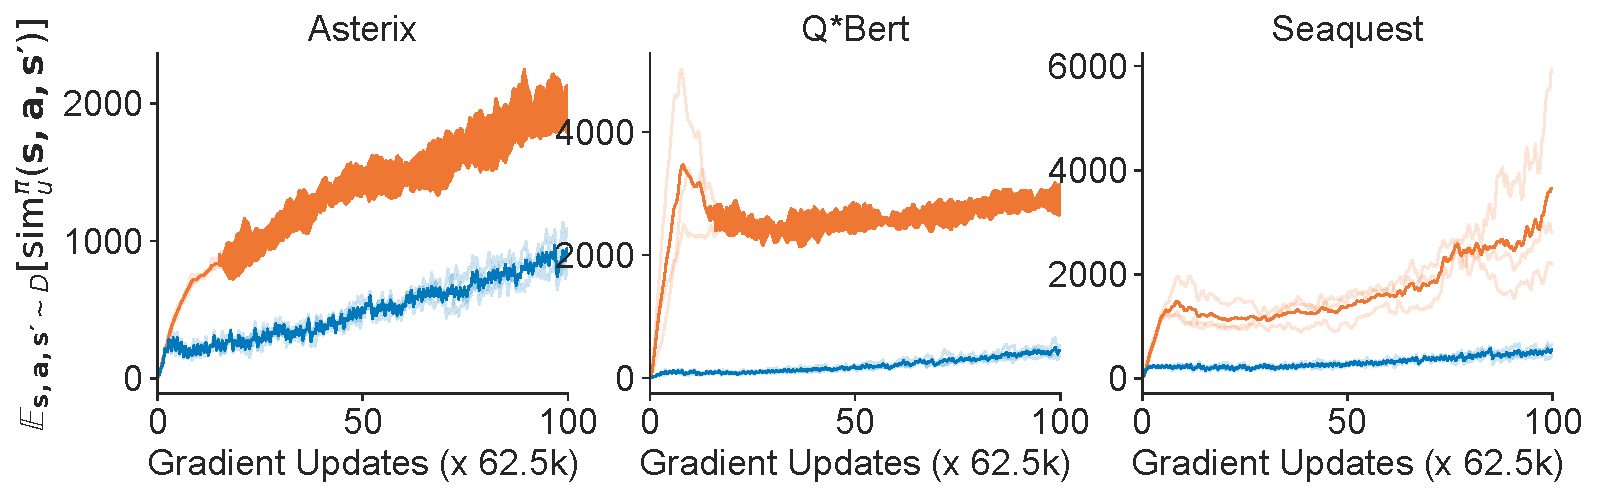
\includegraphics[width=\linewidth]{chapters/dr3/atari/unnorm_3_games.pdf}
    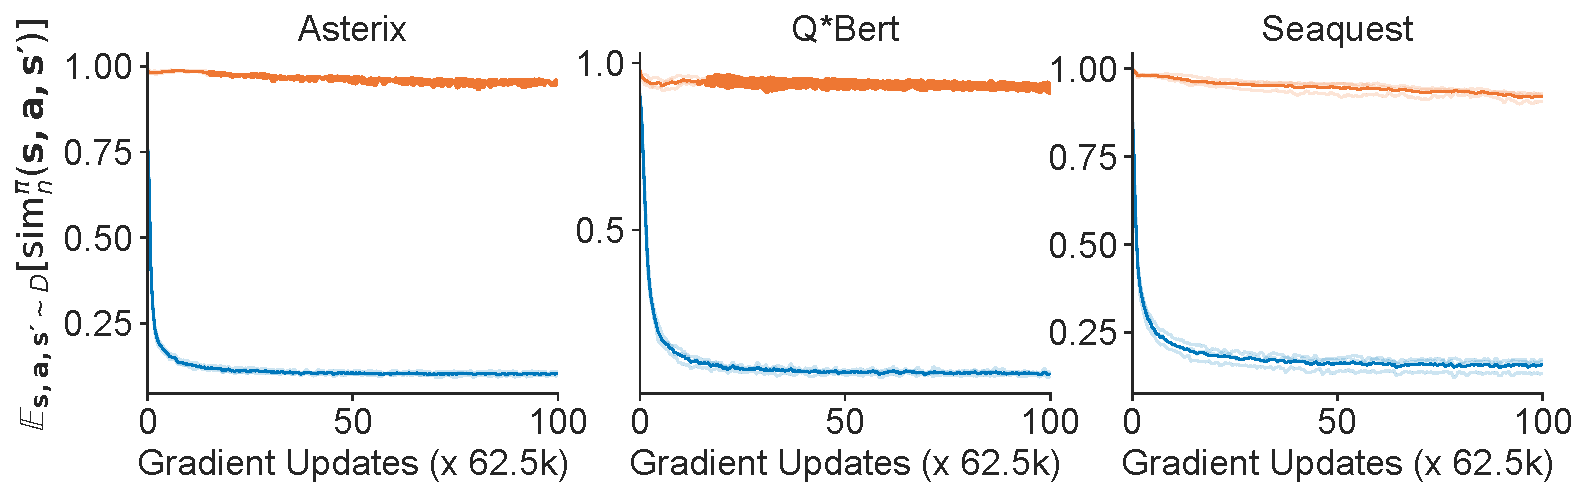
\includegraphics[width=\linewidth]{chapters/dr3/atari/norm_3_games.pdf}
    \vspace{-0.65cm}
    \caption{\small{Performance of offline DQN and BC on 5\% DQN replay dataset~\citep{agarwal2019optimistic} (top), normalized similarity scores for DQN and BC (bottom). As compared to DQN, $\simnorm$ (cosine similarity) decays significantly faster for BC. 
    \textcolor{red}{Remove the middle row that's not useful. Reduce to 2 games. Also add SARSA}}
    } 
    \label{fig:atari_3_games}
    \vspace{-0.4cm}
\end{wrapfigure}
%% The first para is saying aliasing exists in very simple language
%%SL.5.13: I think before we dive into why it happens, can we just show what the problem is? E.g., show some learning curves where performance peaks and drops, and explain what's going on. Only then talk about *why* it happens
%%AK: sorry for bringing this up again. But I feel like that would make it like iUP basically. I have cited this issue of what happens using a figure later in the paper in the para above as well as citing figure from IUP. We can put a wrapfig in the accompanying text above, but it feels a little copied if we spend the technical section on this. Maybe this is not a good choice. What do you think? 
As noted in~\citep{kumar2021implicit}, one of the most notably visible impacts of representation regularization is the pathological feature aliasing phenomenon that arises with more training. While this aliasing issue has been previously quantified via a collapse in the rank of the feature matrix $\Phi$, this evidence does not shed light on the exact mechanism by which aliasing happens -- even standard supervised learning would exhibit a drop in rank($\Phi$); though not in enormous amounts. % one closing line on how as a result it is less clear how to measure aliasing and connection to bootstrapping empirically.   
%%AK: tried to add a comparison against 

\textcolor{red}{This first part of Section 3.1 will likely be removed in favor of a didactic example} \textit{How can we connect the degree of aliasing to bootstrapping?} Since the difference between bootstrapping and standard supervised learning is primarily that the Q-function at $(\bs, \mathbf{a}) \in \mathcal{D}$ is trained  with targets generated using Q-values at $(\bs', \mathbf{a}')$ instead of fixed targets, excessive similarity between $\phi(\bs, \mathbf{a})$ and $\phi(\bs', \mathbf{a}')$ leads to highly coupled Q-values on the two sides of the Bellman update, which can lead to issues such as overestimation and divergence~\citep{durugkar2018td}. Hence, it is informative to measure the similarities in representations $\phi(\bs, \mathbf{a})$ and $\phi(\bs', \mathbf{a}')$. We measure two notions of similarity: \textbf{(1)} we measure the cosine similarity between $\phi(\bs, \mathbf{a})$ and $\phi(\bs', \mathbf{a}')$, and \textbf{(2)} we measure an aggregate    

Observe in  Figure~\ref{fig:atari_3_games} that perhaps surprisingly the similarity between $\phi(\bs, \mathbf{a})$ and $\phi(\bs', \mathbf{a}')$ decreases and saturates at low values with behavior cloning (BC),
%%SL.5.13: This feels like a non-sequitur -- you're comparing representations at two different states, why does it matter that BC is trying to match the behavior policy?
On the other hand, DQN, which is trying to actually improve upon the behavior policy, essentially aliases
%%SL.5.13: There is no evidence of aliasing, just of high dot product (which is not the same)
feature representations at $(\bs, \mathbf{a})$ and $(\bs, \mathbf{a}')$, giving rise to very high similarity values.
%%SL.5.13: Without more context about what's going on, I would say at this point that this is probably due to the OOD actions problem you mentioned before, which DQN does nothing to fix. Additionally, I think it's very likely that many reviewers at this point woudl complain that it's non-sensical to compare BC (which learns policies) with DQN (which learns Q-functions).
This indicates that, compared to supervised learning (e.g., BC), implicit regularization effects in deep Q-learning have a tendency to alias predictions at states and corresponding next states. \textcolor{red}{Would be good to show this with SARSA vs MC: that way we can make a stronger statement like: Note that while both SARSA and MC returns are essentially computing the same quantity and differ only in the nature of implicit regularization induced. This difference makes a huge difference -- in one case, representations at consecutive states are essentially completely aliased, while supervised learning is able to disentangle representations.}
%%SL.5.13: Overall, I think this paragraph is rather problematic. If you want to explain this part, it would be good to really slow it way down and walk the reader through it much more slowly, otherwise so many of the choices in the above paragraph come across as ad hoc, making the conclusions unconvincing.

\fi

\subsection{A Didactic Example}
\label{sec:empirical_analysis}

As noted in~\citep{kumar2021implicit}, one of the most notably visible impacts of representation regularization is the pathological feature aliasing phenomenon that arises with more training. While this aliasing issue has been previously quantified via a collapse in the rank of the feature matrix $\Phi$, this evidence does not shed light on the exact mechanism by which aliasing happens -- even standard supervised learning would exhibit a drop in rank($\Phi$) with more training, and while prior work shows that bootstrapping exacerbates it empirically, it is unclear how exactly this amplification happens. In this section, we describe the intuition behind this mechanism with a didactic example of a 2-action, 1D line MDP~\citep{dong2020expressivity} with a piece-wise linear deterministic dynamics function, $P(\bs'|\bs, \mathbf{a}) = \mathbb{I}(\bs' = f(\bs, \mathbf{a}))$ shown in Figure ??. The reward $r(\bs, \mathbf{a})$ at any state is the value of the state itself, i.e., $r(\bs, \mathbf{a}) = \bs$.

The optimal Q-function for this MDP is shown in Figure ??, and 3-layer deep ReLU network Q-functions estimators learned via supervised regression and TD-learning on the identical finite dataset are shown respectively in Figures ?? and ??. While neither supervised regression nor TD learning can learn the complete structure of the optimal Q-function, TD learning fails to represent important high-frequency components of the Q-function (marked in yellow), leaning a ``simple'', smooth Q-function. Since it fails to model the changes in the Q-function well, the resulting policy often chooses the worse action. Quantitatively, the policy extracted from such a TD Q-function is worse than that extracted from the supervised Q-function at more than half the states.  
%%AK: todo: mark in yellow via keynote

%% The next para is saying aliasing is undesirable
\textbf{Why do we observe overly smooth Q-functions in the didactic example when trained with TD learning?}  While excessive aliasing of internal representations in the neural network is expected to generally lead to poor performance, aliasing between $\phi(\bs, \mathbf{a})$ and $\phi(\bs', \mathbf{a}')$ is especially detrimental when learning with Bellman backups. Intuitively, since Bellman backups train features such that the difference of Q-values, $Q(\bs, \mathbf{a}) - \gamma Q(\bs', \mathbf{a}')$ matches the reward function, $r(\bs, \mathbf{a})$, only on a finite number of state-action tuples seen in the dataset, the features $\phi(\bs, \mathbf{a})$ and $\phi(\bs', \mathbf{a}')$ can learn to only be sufficiently different to predict the reward, thereby achieving low TD error and may be excessively regularized otherwise, thus not capturing long-term structure in the Q-function. Put in other words, there are many possible assignments of weights to a function approximator that could give rise to equally low TD error at the cost of varying degrees of aliasing or regularization.

%%SL.5.13: This feels really hand-wavy. I'm also not sure I agree with this argument -- after all, how would it be any different if there *wasn't* aliasing? Wouldn't you still get a good fit between the difference and reward? This kind of a makes a non-falsifiable statement.
%%AK: this figure is like the example in the MB vs MF paper, but with Bellman backups run on it.

\begin{wrapfigure}{r}{0.5\textwidth}
    \centering
    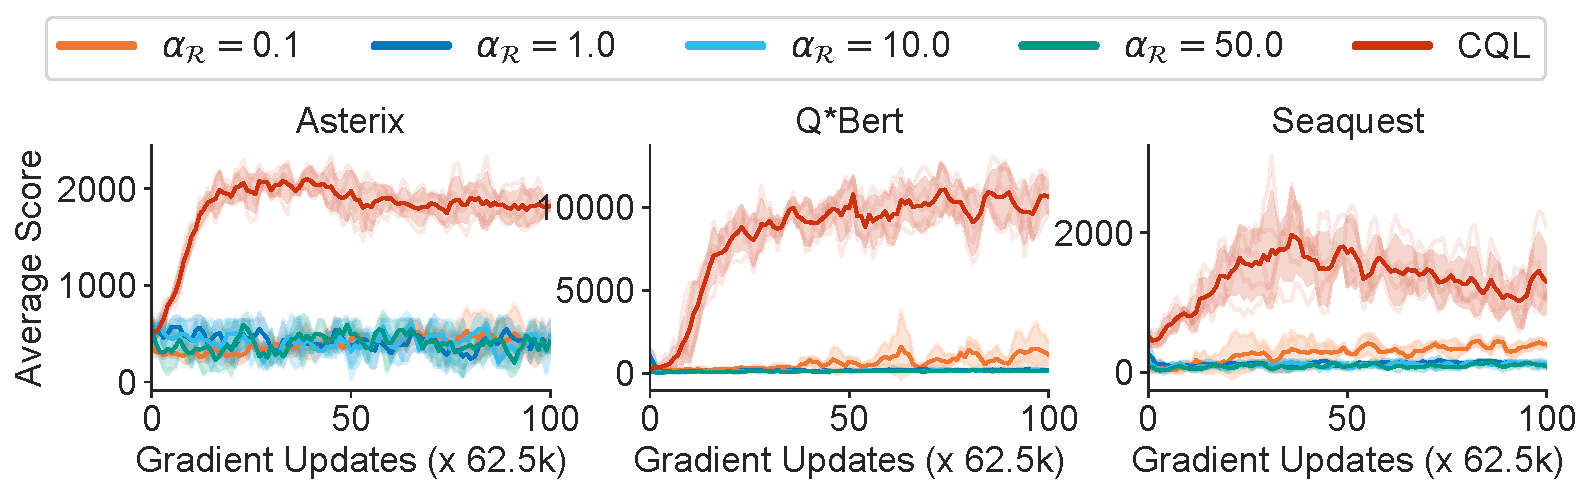
\includegraphics[width=\linewidth]{chapters/dr3/atari/cql_on_bootstrapping_feat.pdf}
    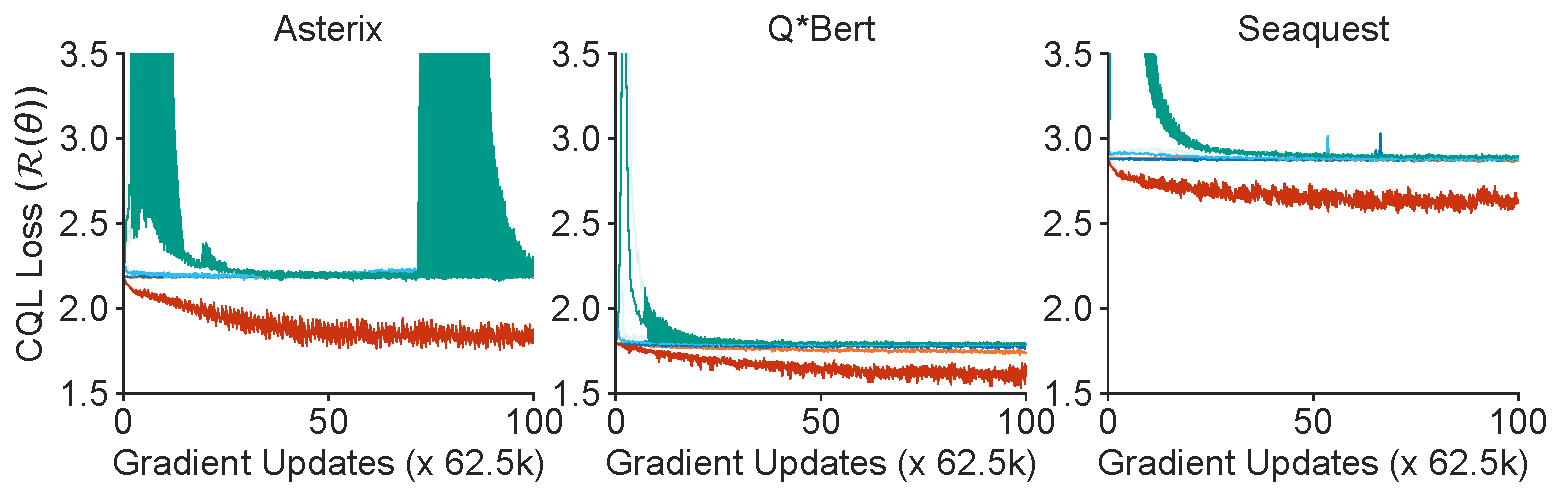
\includegraphics[width=\linewidth]{chapters/dr3/atari/cql_losses_bootstrapped_feat.pdf}
    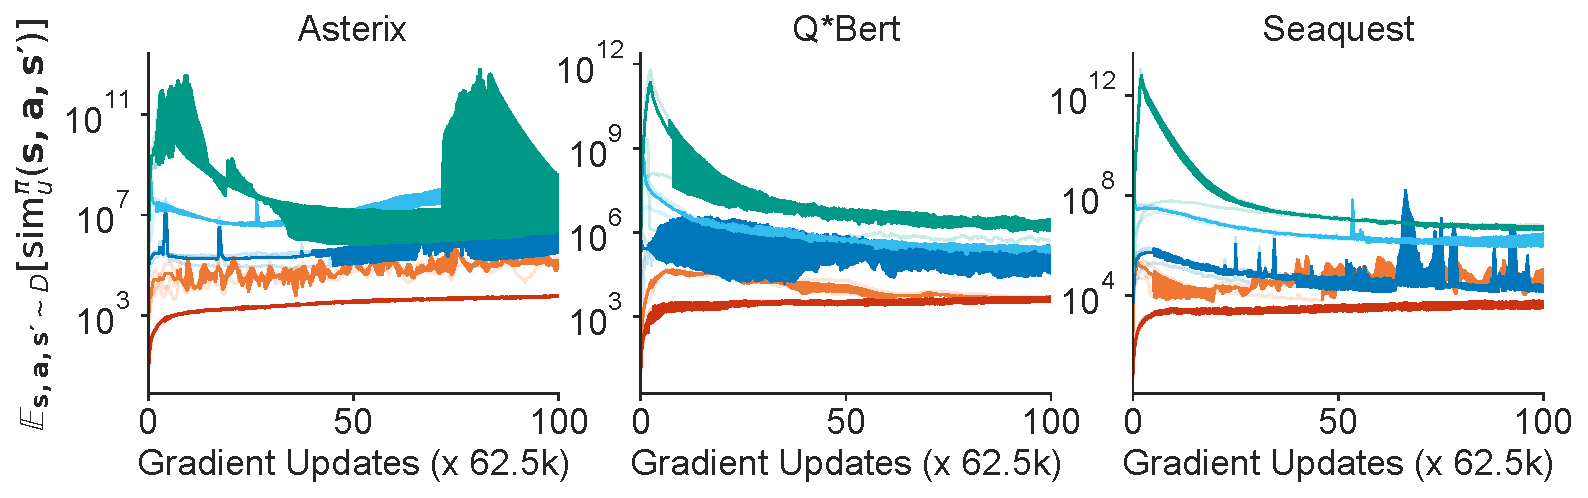
\includegraphics[width=\linewidth]{chapters/dr3/atari/sim_s_ns_cql_on_bootstrapping_feat.pdf}
    \vspace{-0.65cm}
    \caption{\small{CQL($\phi$), trained using 5\% DQN replay dataset, that learns on features trained solely via bootstrapping where the CQL regularizer $\mathcal{R}(\theta)$ only updates the linear weights of the Q-network. Different values of $\alpha_R$ correspond to different strengths of conservative regularization. We also show standard CQL~(red) for comparison.}} 
    \label{fig:atari_3_games_cql_bootstrap}
    \vspace{-0.6cm}
\end{wrapfigure}
When excessive aliasing is induced by such a mechanism, even modern offline RL methods that are meant to prevent against distributional shift
%%SL.5.13: It's unclear what preventing distributional shift has to do with this
are rendered ineffective. To demonstrate this empirically, we trained a modified version of CQL~\citep{kumar2020conservative}, CQL$(\phi)$, that learns on features $\phi(\bs, \mathbf{a})$ solely trained via bootstrapping, and the CQL regularizer is allowed to only update the last linear layer weights. As shown in Figure~\ref{fig:atari_3_games_cql_bootstrap}, no strength of conservative regularization is able to minimize out-of-distribution Q-values resulting in higher values of CQL loss and significantly worse performance as compared to CQL. This indicates that, no matter what, aliased representations can significantly hamper the efficacy of offline RL methods.
%%SL.5.13: This experiment seems weird. You said (and showed before) that features learned with bootstrapping are bad, and it seems like now you are saying if you take those features and retrain, it's still bad, but that's not surprising. I think the subtlety here is that you are also showing that the CQL regularizer is ineffective, but that seems obvious? And it also requires a degree of familiarity with CQL to understand, that the reader might not have. Maybe we can do away with this paragraph?

%%AK: this is the experiment where we initialize the Q-function from a good checkpoint and show it still performs poorly so it is reasoning about the stability aspect.
Finally, to demonstrate the detrimental extent of this implicit regularization on stability of the offline RL algorithm, we perform a controlled experiment where Q-learning is initialized from a ``good'' Q-function that doesn't exhibit aliasing.
%%SL.5.13: where does this come from?
As shown in Figure ??,
%%AK: TODO(AK): add figure!
more learning iterations with modern offline RL algorithms can still drive the algorithm away from this good solution towards more aliased and poor performing solutions. This shows that aliasing caused due to the implicit regularization of training does not just affect the peak performance of an algorithm, but also plays a significant role in destabilizing algorithms when they reach their peak performance.  

\subsection{Theoretical Analysis of Implicit Regularization in Offline Deep Q-Learning}
\label{sec:theory_evidence}
%%SL.5.13: Calling this "implicit regularization" seems premature -- all we showed is that features get larger dot products, which doesn't mean there is some sort of "implicit regularization" going on
In this section, we formalize our empirical observations from Section~\ref{sec:empirical_analysis} and provide a theoretical analysis of the implicit regularization issue. We aim to answer two questions: \textbf{(1)} How do implicit regularization effects in TD learning affect the the aliasing of representations at consecutive states used in the Bellman update? and, \textbf{(2)} How does excessive aliasing affect performance of the algorithm? To answer these questions, we first introduce a simple abstract model of neural network behavior
%%SL.5.13: Rephrase as something like: we first introduce a simple abstract model of neural network training dynamics in value-based RL, and then use this model to analyze the effect of repeated SGD updates on the TD objective. [or something like that]
that allows us to answer these questions.

% abstract model
%% AK: TODO (AK): Also check if we can generalize this to arbitrary continous domains
%%SL.5.13: In its current form, I'm a bit nervous about this version of the theory. I think the SGD implicit regularization version is more convincing and makes fewer arbitrary choices. I do think this version could be made better if we can get rid of the discrete set though. Would be good to get Tengyu's take on it too...
\textbf{Abstract model.} Our abstract model captures feature learning as making a discrete selection among $K$ different feature vector candidates, $\{\Phi_1, \Phi_2, \cdots, \Phi_K\}$, $\Phi_i \in \mathbb{R}^{|\data|\times d}$,
%%SL.5.13: It would be way easier to understand if we could get continuous domains, and then just frame this as an optimization over \Phi (i.e., optimization over \Phi corresponds to selecting the best \Phi \in [some set]), that way we don't have to have this "discrete selection" business and could just say that it's part of the optimization process.
and then training a linear layer $\bw \in \mathbb{R}^{d}$ to obtain the Q-function.
%%SL.5.13: One way you could phrase is this: Our abstract model of the learning process separates the neural network into two parts: a representation $\Phi$ and a weight vector $\bw \in ...$, such that the full model is given by $\Phi(..)^T \bw$ (i.e., $\bw$ corresponds to the last linear layer). The learning process is framed as a \emph{bilevel} optimization problem, where the weights $\bw$ are chosen subject to a constraint that the learning process chooses the optimal features $\Phi \in [set]$ for $\bw$ (or something like that)
To mimic the overparameterized nature of neural networks, we assume that we operate in the overparameterized regime with $n < d$.
%%SL.5.13: This is kind of weird -- usually the last layer features are not that high dimensional, but the model parameters are. Are you sure we shouldn't look for some way to "NTK-ify" this? Perhaps a better way to frame this is that we are in the NTK regime where the choice of Phi corresponds to the choice of NTK (i.e., it's not fixed, as is more common in this analysis), while bw corresponds to the neural net parameters? That would justify the overparameterized regime and make this less weird.
Assume that the initial value of the weight vector $\bw^{(0)} = 0$. We then write out the minimum-norm optimization problem shown below in Equation~\ref{eqn:min_norm} that attains the same solution as the optimal solution found by minimizing training TD error in this model, and characterize the properties of features $\Phi_K^*$ that are selected to obtain the minimum-norm solution. \textcolor{red}{more assumptions?}     
%%SL.5.13: It won't be clear to some people what min-norm has to do with neural net training, can you cite something to justify this?
\begin{align}
    \min_{\bw, \boldm_i \in \{0^d, 1^d \}}~~& ||\bw||_2^2 \nonumber\\
    \text{s.t.}~~&~ \mathbf{a}r{\Phi}^\top \mathbf{a}r{\Phi} \bw = \mathbf{a}r{\Phi}^\top R + \gamma \mathbf{a}r{\Phi}^\top P^\pi \mathbf{a}r{\Phi} \bw, ~~ \mathbf{a}r{\Phi} = \left[\Phi_1, \cdots, \Phi_k\right] \otimes [\boldm_1, \cdots, \boldm_K]
\label{eqn:min_norm}
\end{align}
%%SL.5.13: ouch, this \bm_i is... difficult to parse
Our first result characterizes the feature representation $\mathbf{a}r{\Phi}$ -- equal to one of $\Phi_i$ selected based on the learned masks $\bm_i$ -- that satisfies the Bellman consistency condition but also minimize the implicit regularizer, $||\bw||_2^2$,
%%SL.5.13: where does this implicit regularizer come from?
and use this to depict the existence of this phenomenon.

\begin{theorem}
\label{thm:aliasing_exists}
Let the singular value decomposition of $\Phi_i$ be given as $\Phi_i = \bU_i \Sigma_i \bV_i^\top$ and $\bw^{(*)}, \boldm^{(*)}$ minimize the objective in Equation~\ref{eqn:min_norm}. Assume that the reward vector lies in the column space of $\Phi_i$, $\forall i \in [K]$, i.e., $\exists~ y_i, R = \Phi_i y_i $.  Then, $\mathbf{a}r{\Phi}$ is such that:
\begin{equation*}
    \mathbf{a}r{\Phi} := \arg \min_{i}~ \big|\big| \Sigma_i^{-1} \left( \bU_i^T (I - \gamma P^\pi) \bU_i \right)^{-1} \Sigma_i y_i\big|\big|_2^2.
\end{equation*}
Thus, the resulting $\mathbf{a}r{\Phi}$ satisfies: $\mathrm{srank}\left(\mathbf{a}r{\Phi}^\top (\mathbf{a}r{\Phi} - \gamma P^\pi \mathbf{a}r{\Phi}) \right) \leq \mathrm{srank}\left(\Phi_i^\top (\Phi_i - \gamma P^\pi \Phi_i) \right)~ \forall i$, which quantifies the existence of aliasing between representations at consecutive states in TD-learning.
\end{theorem}
%%SL.5.13: It's not clear what this last sentence means ("which quantifies the existence of aliasing between representations at consecutive states in TD-learning") -- can we state the implication of this theorem more precisely. As written, it's also not clear what this theorem has to do with SGD (I guess it's the min-norm part?).

%%SL.5.13: It might also help with clarity to explain why this problem *doesn't* happen in the supervised learning case

A proof of Theorem~\ref{thm:aliasing_exists} can be found in the Appendix ??. The main consequence of this result is a characterization of the learned features at optimal TD solutions in our abstract model in terms of the effective rank~\citep{kumar2021implicit} of the matrix $\bM(\Phi) := \Phi^\top (\Phi - \gamma P^\pi \Phi)$. A low rank of $\bM(\Phi)$ for a given rank of $\Phi$ intuitively indicates that the basis of the difference in features at consecutive states, $\Phi - \gamma P^\pi \Phi$, heavily lies
%%SL.5.13: try to avoid hand-wavy language ("heavily lies") and state what you mean more precisely
in the null space of the feature matrix $\Phi$, as a result of which the weight vector $\bw$ will be updated only in a few directions allowed by both $\Phi$ and $\Phi-\gamma P^\pi \Phi$.indicating that only a partial set of features will actually be used for learning.
%%SL.5.13: something is malformed above ("indicating that")
To empirically verify the existence of such an aliasing phenomenon, following the procedure outlined in \citep{kumar2021implicit}, we measure the effective rank of $\bM(\Phi)$ and observe in Figure ?? that this matrix indeed has extremely low rank when training with TD backups, as compared to supervised regression.
%% AK: this supervised regression is BC. Should we also do this for something else?

%%AK: maybe write the stuff below as a theorem?
Another interesting consequence of Theorem~\ref{thm:aliasing_exists} is the effect of the ``simplicity'' of the reward function on feature aliasing. We define simplicity by the number of non-zero components in the vector $y_i$.
%%SL.5.13: maybe we should avoid ad hoc definitions like this, and try to just state this more plainly and directly?
As an extreme case, note that if the vector $y_i$ has all zeros, except a single 1 entry, the optimal $\mathbf{a}r{\Phi}$ is expected to induce $\bM(\Phi)$ with a much lower rank compared to when a significantly more number of values of $y_i$ are non-zero (as shown in Appendix ??).
%%SL.5.13: this seems imprecise ("much lower")
This means that when the reward function $R$ actually non-trivially combines the singular vectors of $\Phi$ -- which we refer to as a ``complex'' reward function -- the effective aliasing
%%SL.5.13: I think if you're going to use the term "aliasing" like this, it needs to be formally defined. Aliasing means that two things are indistinguishable (not similar, but indistinguishable). The word is being used in a different way here.
is little less than when it does not. We indeed observe this behavior in practice, as shown in Figure ?? in Section~\ref{sec:empirical_analysis}, and our abstract model sheds light on how this implicit regularization effect in TD-learning is exacerbated in scenarios where reward functions can be expressed using very few components of the feature matrix $\Phi$.
%%SL.5.13: how do you know if it can be expressed using very few components?
%%SL.5.13: I think I understand what you are trying to say in the above paragraph, but we need to find a cleaner and more concise way of saying it. Maybe what we can say is something like -- consider the projection of the reward function onto the column-space [?] of Phi, with coefficients ??. If these coefficients are sparse, we would expect [??] (try to be precise!)...

To conclude our analysis for question \textbf{(1)}, we finally note that an analogous result in supervised learning would indicate no existence of any implicit bias that preferentially aliases feature representations at consecutive states. While prior work \citep{kumar2021implicit} has also generally shown the compounding effect of implicit regularization towards low-rank $\Phi$ in TD-learning, our analysis explicitly identifies the structure of aliasing induced by this implicit regularization: the rank of the matrix $\bM(\phi)$ drops, leading to aliasing at consecutive states.
%%SL.5.13: It's good to have a paragraph like the one above, but it addresses two things simultaneously, and doesn't do either very well: the supervised learning bit seems to have no punchline (so... is this a contradiction? if not, why not?); the bit about IUP doesn't clearly state how what you are showing is different from IUP.

%%SL.5.13: Given how long-winded the above is, maybe consider a subsection heading for (2) or something (or at least paragraph heading)
Next, we answer question \textbf{(2)} regarding the detrimental impacts of aliasing. 
\textcolor{red}{Need to finish this bit -- there are some options we can go: (1) We can show that there exist MDPs with simple reward functions and complex Q-functions, where such an implicit regularizer will cause the MDP to learn overly smooth Q-functions. (2) We can show that even when initialized close to a good solution, this implicit regularizer will drive the model towards picking features that are the most aliased, in which case we do not even stabilize near a good solution even if we reach it. (3) We could show that distributional shift correction on top of aliased features will not work, similar to what we had before the ICML deadline. Which of these option(s) should we prefer?}

\fi